% Emerald Publishing - Construction Innovation Submission Template
% by Oleksandr Melnyk
% Ver 0.0.4
% Based on: https://www.emeraldgrouppublishing.com/journal/ci#author-guidelines


\documentclass[12pt]{article}
\usepackage{setspace}
\onehalfspacing
\usepackage[english]{babel}
\usepackage{appendix}
\usepackage{tikz}
\usetikzlibrary{patterns}
\usepackage{standalone}

% Set page size and margins
% Replace `letterpaper' with `a4paper' for UK/EU standard size
\usepackage[a4paper,top=2cm,bottom=2cm,left=3cm,right=3cm,marginparwidth=1.75cm]{geometry}

\usepackage{sectsty}
\sectionfont{\fontsize{15}{15}\selectfont}

% Useful packages
\usepackage{amssymb,amsmath}
\newtheorem{theorem}{Theorem}
\newtheorem{proposition}{Proposition}
\newtheorem{lemma}{Lemma}
\newtheorem{corollary}{Corollary}
\newtheorem{remark}{Remark}
\usepackage{siunitx}
\PassOptionsToPackage{hyphens}{url}\usepackage{hyperref}
\usepackage{cleveref}
\usepackage[utf8]{inputenc}
\usepackage[left]{lineno}
\usepackage{csquotes}
\usepackage{booktabs}
\usepackage{longtable}
\usepackage{adjustbox}
\usepackage{array}
\usepackage{url}
\usepackage{titlesec}
%\usepackage[compatibility=false]{caption}
\usepackage{authblk}
\usepackage{xcolor} % Load the xcolor package for color options
\renewcommand{\thetable}{\Roman{table}}

% Define a new format for \subsection
\titleformat{\subsection}
  {\mdseries\itshape\large} % Medium series, italic shape, and large font size
  {\thesubsection}{1em}{} % Numbering, spacing, and the section title itself


% Emerald Harvard Citation Style

\usepackage[style=authoryear,backend=biber,natbib=true,maxcitenames=2,uniquelist=false,url=false,doi=false,eprint=false,isbn=false]{biblatex}
\addbibresource{refer.bib} % your .bib file
\addbibresource{AI.bib} % your .bib file

% Customizing biblatex for Harvard style
% Customizing biblatex for Harvard style
\DeclareNameAlias{sortname}{family-given}
\DeclareNameAlias{default}{family-given}

\renewbibmacro{in:}{}
\DeclareFieldFormat[article]{title}{\mkbibquote{#1}\addcomma}
\DeclareFieldFormat[book]{title}{\mkbibemph{#1}\addcomma}
\DeclareFieldFormat[bookinbook]{title}{\mkbibemph{#1}\addcomma}
\DeclareFieldFormat[inbook]{title}{\mkbibquote{#1}\addcomma}
\DeclareFieldFormat[incollection]{title}{\mkbibquote{#1}\addcomma}
\DeclareFieldFormat[inproceedings]{title}{\mkbibquote{#1}\addcomma}
\DeclareFieldFormat[manual]{title}{\mkbibemph{#1}\addcomma}
\DeclareFieldFormat[misc]{title}{\mkbibemph{#1}\addcomma}
\DeclareFieldFormat[thesis]{title}{\mkbibemph{#1}\addcomma}
\DeclareFieldFormat[unpublished]{title}{\mkbibquote{#1}\addcomma}
\DeclareFieldFormat[patent]{title}{\mkbibemph{#1}\addcomma}
\DeclareFieldFormat[report]{title}{\mkbibemph{#1}\addcomma}
\DeclareFieldFormat[online]{title}{\mkbibquote{#1}\addcomma}
\DeclareFieldFormat[software]{title}{\mkbibemph{#1}\addcomma}
\DeclareFieldFormat[booklet]{title}{\mkbibemph{#1}\addcomma}
\DeclareFieldFormat[periodical]{title}{\mkbibemph{#1}\addcomma}
\DeclareFieldFormat[standard]{title}{\mkbibemph{#1}\addcomma}

\DeclareFieldFormat[article]{journaltitle}{\iffieldundef{shortjournal}{\mkbibemph{#1}\addcomma}{\mkbibemph{\printfield{shortjournal}}\addcomma}}
\DeclareFieldFormat{volume}{\bibstring{volume}~#1}
\DeclareFieldFormat{number}{\bibstring{number}~#1}

% Definitions for "Vol." and "No."
\DefineBibliographyStrings{english}{
  volume = {Vol.},
  number = {No.}
}

\renewbibmacro*{volume+number+eid}{%
  \printfield{volume}%
  \setunit*{\addspace}%
  \printfield{number}%
  \setunit{\addcomma\space}%
  \printfield{eid}}

\renewbibmacro*{journal+issuetitle}{%
  \usebibmacro{journal}%
  \setunit*{\addcomma\space}%
  \usebibmacro{volume+number+eid}%
  \setunit{\addcomma\space}%
  \usebibmacro{issue+date}}

\renewbibmacro*{publisher+location+date}{%
  \printlist{publisher}%
  \iflistundef{location}
    {\setunit*{\addcomma\space}}
    {\setunit*{\addcolon\space}}%
  \printlist{location}%
  \setunit*{\addcomma\space}%
  \usebibmacro{date}}

\renewcommand*{\bibpagespunct}{\addcomma\space}

\newcommand\YL[1]{\textcolor{blue}{YL: #1}}	

% Customizing page field format to prevent duplication
% \DeclareFieldFormat{pages}{%
%   \mkfirstpage[{\mkpageprefix[page]{#1}}]{#1}}

% Customizing citations for Harvard style
\DeclareCiteCommand{\cite}[\mkbibparens]
  {\usebibmacro{prenote}}
  {\usebibmacro{citeindex}%
   \usebibmacro{cite}}
  {\multicitedelim}
  {\usebibmacro{postnote}}

\renewbibmacro*{cite:labelyear+extrayear}{%
  \iffieldundef{labelyear}
    {}
    {\printtext[bibhyperref]{%
       \printfield{labelyear}%
       \printfield{extrayear}}}}

\renewbibmacro*{cite:labeldate+extradate}{%
  \iffieldundef{labelyear}
    {}
    {\printtext[bibhyperref]{%
       \printfield{labelyear}%
       \printfield{extradate}}}}

\AtEveryBibitem{
  \clearfield{month}
  \clearfield{day}
  \ifentrytype{book}{
    \clearlist{location}
  }{}
}

% Formatting "et al." in italics followed by a comma
\DefineBibliographyStrings{english}{
  andothers = {\textit{et al.},}
}

\DeclareFieldFormat[article]{volume}{\bibstring{jourvol}\addnbspace #1}
\DeclareFieldFormat[article]{number}{\bibstring{number}\addnbspace #1}
\DeclareFieldFormat[article]{volume}{Vol. #1}
\DeclareFieldFormat[article]{number}{No. #1}
% Customizing DOI field format to lowercase "doi"
%\DeclareFieldFormat{doi}{\bibstring{doi}\addcolon\space\url{#1}}

% % Customizing URL field format to "available at:"
% \DeclareFieldFormat{url}{\bibstring{available at}\addcolon\space\url{#1}}
% \DeclareFieldFormat{urldate}{\mkbibparens{accessed \addspace#1}}

% % Customizing urldate to match the required format
% \DeclareFieldFormat{urldate}{%
%   \mkbibparens{accessed\space%
%     \thefield{urlday}\addspace%
%     \mkbibmonth{\thefield{urlmonth}}\addspace%
%     \thefield{urlyear}}}


% Configure cleveref
%\crefformat{figure}{#2Figure~#1#3}
%\Crefformat{figure}{#2Figure~#1#3}
%\crefformat{table}{#2Table~#1#3}
%\Crefformat{table}{#2Table~#1#3}
\crefformat{section}{#2Section~#1#3}
\Crefformat{section}{#2Section~#1#3}

%Front Matter
\author[1]{Yang K. Lu}
\author[2]{Eunseong Ma}

\affil[1]{HKUST}
\affil[2]{Yonsei}

%\title{\Large Anticipating AI-Driven Skill Demand: Human Capital Responses and Macro-Level Implications}
\title{\LARGE AI and Human Capital Accumulation: \\ Aggregate and Distributional Implications\footnote{Author emails: yanglu@ust.hk; masilver@yonsei.ac.kr}}


\begin{document}
\maketitle


\begin{abstract}
This paper develops a model to analyze the effects of AI advancements on human capital investment and their impact on aggregate and distributional outcomes in the economy. We construct an incomplete markets economy with endogenous asset accumulation and general equilibrium, where households decide on human capital investment and labor supply. Anticipating near-term AI advancements that will alter skill premiums, we analyze the transition dynamics toward a new steady state. Our findings reveal that human capital responses to AI amplify its positive effects on aggregate output and consumption, mitigate the AI-induced rise in precautionary savings, and stabilize the adjustments in wages and asset returns. Furthermore, while AI-driven human capital adjustments increase inequalities in income, earnings, and consumption, they unexpectedly reduce wealth inequality.\\
\\
%add 6 keywords
\textbf{Keywords:} AI, Job Polarization, Human Capital, Inequality
\end{abstract}
\linenumbers

\newpage

\section{Introduction}
\label{sec:introduction}

The distinctive nature of AI advancements lies in their ability to perform cognitive, non-routine tasks that previously required significant education and expertise, fundamentally differentiating its impact on the labor market and economy from that of general automation. For example, AI tools in medical diagnostics now assist radiologists in analyzing medical images, potentially reducing demand for entry-level radiologists while simultaneously increasing the productivity of senior professionals. More generally, AI could shift the premium associated with various skills levels, devaluing middle-level skills while increasing the demand for high-level expertise. In anticipation of these changes, households are likely to adjust their human capital investments.


According to the National Center for Education Statistic,\footnote{\url{https://nces.ed.gov/programs/digest/d22/tables/dt22_303.70.asp}} college enrollment in the U.S. has been declining since 2010. The National Student Clearinghouse Research Center reports that the undergraduate college enrollment decline has accelerated since the pandemic began, resulting in a loss of almost 6\% of total enrollment between fall 2019 to fall 2023, while graduate enrollment has risen by about 5\%.\footnote{\url{https://public.tableau.com/app/profile/researchcenter/viz/CTEEFall2023dashboard/CTEEFall2023}} These shifts, regardless of their causes, highlight evolving patterns in human capital investment. 


This paper develops a model to study the effects of AI advancements on human capital investment and their subsequent impact on aggregate and distributional outcomes of the economy. We posit an economy consisting of three sectors, requiring low, middle and high levels of skill (human capital) with increasing sectoral labor productivity. Households can invest in their human capital to move up to more productive sectors. But if they do not invest, their human capital depreciates and, over time, they will move down to less productive sectors. We model human capital investment at two levels, a low level attainable on the job and a high level requiring full-time commitment, such as pursuing higher education. Households are subject to uninsurable idiosyncratic risk in terms of productivity shocks that affect both labor productivity and effectiveness in human capital investment. 


The interaction between human capital investment and labor supply presents a tradeoff at the household level between current wage earning and future wage gains. At aggregate level, the interaction implies that when individuals transition from the middle to the high sector, they may temporarily exit the workforce to upskill, reducing immediate labor supply but improving future labor productivity. 


We model AI advancements as increasing the productivity for the low and high sectors but not for the middle sector so that the skill premium of the middle sector decreases and the skill premium of the high sector increases. Allowing for human capital adjustments not only alters AI’s economic implications quantitatively, it also makes a qualitative difference. 


If the skill distribution is fixed, AI will unambiguously improve the labor productivity of the whole economy. However, allowing human capital to adjust enables workers to upskill or downskill. The response of overall labor productivity could be enhanced, or dampened, or even reverted depending on whether workers move to more or less productive sectors.


Using a two-period model, we show how households’ labor supply and human capital investment are affected by their productivity shocks, asset holdings and stocks of human capital. The effects of AI, in this partial equilibrium analysis, are shown to discourage human capital investment for households in the low sector and encourage human capital investment for households in the middle sector, thereby increasing human capital inequality. In addition, AI worsens consumption inequality for households with low levels of human capital and reduces consumption inequality for those with high levels of human capital.


At the economy level, the effects of AI advancements depend on the sectoral distribution of households and the general equilibrium effects via wage and capital return responses. We quantify these effects using a fully-fledged dynamic quantitative model that incorporates an infinite horizon, endogenous asset accumulation, and general equilibrium. The model is calibrated to reflect key features of the U.S. economy, capturing
realistic household heterogeneity. The steady state distribution of human capital without AI advancements pins down the sectoral distribution of households. We then introduce fully anticipated AI advancements happening in the near future and study the transition dynamics from the current state of the economy to the eventual new steady state. 

We find that aggregate human capital rises sharply even before AI introduction, indicating that a substantial portion of workers, anticipating changes in skill premium, leave the labor force early to accumulate human capital. The economy also experiences AI-induced job polarization, with a notable reallocation of workers from the middle sector to either low or high sectors.

Building on these labor dynamics, our model examines how AI influences both the aggregate and distributional outcomes of the economy, including output, consumption, investment, employment, income inequality, consumption inequality, and wealth inequality. Our focus is on how human capital adjustments reshape AI’s effects on each of these outcomes. Specifically, we examine two primary channels through which human capital adjustments operate: the redistribution channel, which reallocates workers across skill sectors, and the general equilibrium channel, which operates through wages and capital return changes.

Our findings reveal that human capital responses to AI amplify its positive effects on aggregate output and consumption, mitigate the AI-induced rise in precautionary savings, and stabilize the adjustments in wages and asset returns. Furthermore, while AI-driven human capital adjustments increase inequalities in income, earnings, and consumption, they unexpectedly reduce wealth inequality. We also show that the redistribution channel is the dominant factor in the effects of human capital adjustments, whereas the general equilibrium channel, via wage and capital return changes, plays a comparatively minor role.

%Suppose that labor supply declines as a result of households in the middle sector exiting the workforce to invest in their human capital in anticipating the AI advancements. The equilibrium wage will increase, disproportionately benefiting high-sector workers whose labor produces more effective units. This will encourage further shifts from the middle sector and amplifying human capital adjustments.

INTRODUCING PRECAUTIONARY SAVING MOTIVE IN THE WAGE POLARIZATION INVESTIGATION \citet{autor_polarization_2006}


This paper relates to the literature examining how technological advancements,
including AI, have significantly contributed to job polarization.
\citet{Goos2007} show that since 1975, the United Kingdom has experienced
job polarization, with increasing employment shares in both high-
and low-wage occupations. \citet{Autor2013} expanded on this by providing
a unified analysis of the growth of low-skill service occupations,
highlighting key factors that amplify polarization in the U.S. labor
market. Empirical evidence from \citet{Goos2014} further confirms
pervasive job polarization across 16 advanced Western European economies.
In the U.S., \citet{Acemoglu2020} show that robots can reduce employment
and wages, finding robust negative effects of automation on both in
various commuting zones.

The introduction of AI and robotics has had adverse effects on labor
markets, with significant implications for employment and labor force
participation. \citet{Lerch2021} highlights that the increasing use
of robots not only displaces workers but also negatively impacts overall
labor force participation rates. Similarly, \citet{Faber2022} demonstrate
that the detrimental effects of robots on the labor market have resulted
in a decline in job opportunities, particularly in sectors where automation
is prevalent. These findings suggest that while technological advancements
bring productivity gains, they simultaneously reduce employment prospects
and participation in the labor market, exacerbating economic challenges
for certain groups of workers.

The introduction of AI and robotics also influences human capital
accumulation as workers respond to technological disruption. Faced
with the employment risks brought about by automation, many exposed
workers may invest in additional education as a form of self-insurance,
rather than relying on increases in the college wage premium \parencites{Atkin2016,Beaudry2016}. Empirical evidence supports this response.
\citet{DiGiacomo2023} find that for every additional robot adopted
in U.S. local labor markets between 1993 and 2007, four individuals
enrolled in college, particularly in community colleges, indicating
a rise in educational investments triggered by automation. Similarly,
\citet{Dauth2021} show that within German firms, robot adoption has
led to an increase in the share of college-educated workers, as firms
prioritize higher-skilled employees over those with apprenticeships. 

The response of human capital accumulation to technological disruption could also go to the other extreme. A 2022 report by Higher Education Strategy Associates finds that following decades of growth, dropping student enrollment has become a major trend in higher education in the Global North.\footnote{\url{https://higheredstrategy.com/world-higher-education-institutions-students-and-funding/}} In the U.S., the public across the political spectrum has increasingly lost confidence in the economic benefits of a college degree. Pew Research Center reports that about half of Americans say having a college degree is less important today than it was 20 years ago in a survey conducted in 2023.\footnote{\url{https://www.pewresearch.org/social-trends/2024/05/23/public-views-on-the-value-of-a-college-degree/}} A 2022 study from Public Agenda, a nonpartisan research organization, shows that young Americans without college degrees are most skeptical about the value of higher education.


The rise of AI and automation also plays a significant role in exacerbating
general inequality, particularly through its impact on education and
wealth distribution. \citet{Prettner2020} present a model showing
that innovation-driven growth leads to an increasing proportion of
college graduates, which in turn drives higher income and wealth inequality.
As technology advances, workers with higher educational attainment
benefit disproportionately, widening the gap between those with and
without advanced skills. \citet{Sachs2012} also explore this dynamic,
providing a model within an overlapping generations framework that
examines the interaction between automation and education. They demonstrate
how automation can further entrench inequality by favoring workers
with higher levels of education, as those without adequate skills
are more likely to be displaced or see their wages stagnate. This
interaction between technological change and educational attainment
not only amplifies economic inequality but also perpetuates disparities
in wealth across generations.

The rest of the paper is organized as follows. Section 2 describes the model environment. Section 3 solves the household's problem using a two-period version of the model. Section 4 solves the fully-fledged quantitative model and calibrates it to fit key features of the U.S. economy, including employment rate, human capital investment, and household heterogeneity. Section 5 incorporates AI into the quantitative model and examines its economic impact on both aggregate and distributional outcomes. Section 6 analyzes how human capital adjustments change the economic impact of AI advancements. Section 7 concludes.

\section{Model Environment }
\label{sec:model}
Time is discrete and infinite. 
There is a continuum of households. Each household is endowed with one unit of indivisible labor and faces idiosyncratic productivity shock, $z$, that follows an AR(1) process in logs:
\begin{equation}
    \label{eq:z}
\ln z'=\rho_z\ln z + \varepsilon_z, \varepsilon_z \overset{\mathrm{iid}}{\sim} N(0,\sigma_z^2)
\end{equation}
The asset market is incomplete following \citet{aiyagari_uninsured_1994}, and the physical capital, $a$, is the only asset available to households to insure against this idiosyncratic risk. Households can also invest in human capital, $h$, which allows them to work in sectors with different human capital requirement.

\subsection{Production Technology}
The production technology in the economy is a constant-returns-to-scale Cobb-Douglas production function:
\begin{equation}
    F(K,L)=K^{1-\alpha} L^{\alpha}
\end{equation}
$K$ is the aggregation of all physical capital held by the households. $L$ is the aggregation of effective labor supplied by the households and employed in three sectors: low, middle, and high. 

These sectors differ in their technologies for converting labor into effective labor units and in the levels of human capital required for employment. 
The middle sector employs households with human capital above $h_M$ and converts one unit of labor to one effective labor unit. The high sector, requiring human capital above $h_H$, converts one unit of labor to $1+\lambda$ effective units, while the low sector, with no human capital requirement, converts one unit into $1-\lambda$ effective units. This implies a sectoral labor productivity $x(h)$ that is a step function in human capital:
\begin{equation}
    \label{eq:x}
x(h)=\left \{ 
\begin{array}{cl}
1-\lambda  & \text{low sector if }h<h_{M} \\ 
1 & \text{middle sector if }h_{M}<h<h_{H} \\ 
1+\lambda  & \text{high sector if }h>h_{H}%
\end{array}%
\right. 
\end{equation}
A household $i$ who decides to work thus contributes $z_ix(h_i)$ units of effective labor, where $z_i$ is his idiosyncratic productivity. Denote $n_i \in \{0,1\}$ as the indicator that takes one if the household works and zero if the household does not. The aggregate labor is
\begin{equation}
    L=\int n_iz_ix(h_i)di,
\end{equation}
assuming perfect substitutability of effective labor across the three sectors.

\subsection{Household's Problem}
Households derive utility from consumption, incur disutility from labor and effort of human capital investment. 
A household maximizes the expected lifetime utility by optimally choosing consumption, saving, labor supply and human capital investment each period, based on his idiosyncratic productivity shock $z_t$:
\begin{equation}
\max_{\left \{ c_t,a_{t+1},n_t,e_t\right \}_{t=0}^{\infty }}E_0\left[
\sum\limits_{t=0}^{\infty }\beta^t( \ln c_t-\chi_n n_t-\chi_e e_t ) \right] 
\end{equation}
where $c_t$ represents consumption, $a_{t+1}$ represents saving, $n_t \in \{0,1\}$ is labor supply, and $e_t$ is the effort of human capital investment.

If a household decides to work in period $t$, he will be employed into the appropriate sector according to his human capital $h_t$ and receive labor income $w_tz_tx(h_t)$, where $w_t$ is the economy-wide wage rate of effective labor unit.

Denote $r_t$ as the interest rate on the physical capital $a_t$. The household's budget constraint is
\begin{align}
    c_t+a_{t+1}&=n_t( w_tz_tx(h_t))+(1+r_t)a_t \\
    c_t& \geq 0 \text{ and } a_{t+1} \geq 0
\end{align}
We prohibit households from borrowing $a_{t+1} \geq 0$ to simplify analysis.\footnote{According to \citet{aiyagari_uninsured_1994}, a borrowing constraint is necessarily implied by present value budget balance and nonnegativity of consumption. Since the borrowing limit is not essential to our analysis, we set it to zero for simplicity.} 

Human capital investment can take three levels of effort: $\{0,e_L,e_H\}$. A non-working household is free to choose any of the three effort levels but a working household cannot devote the highest level of effort $e_H$, reflecting a trade-off between working and human capital investment. Hence:
\begin{equation}
e_t \in \{0, e_L, (1-n_t)e_H\}.
\end{equation}
Its contribution to next-period human capital is subject to the productivity shock:
\begin{equation}
h_{t+1}=z_te_t + (1-\delta)h_t
\end{equation}
where $\delta$ is human capital's depreciation rate. 
 
\section{Household Decisions in a Two-Period Model}
In this section, we solve the household's problem with two periods to gain intuition. 


\subsection{Period-2 Decisions}\label{sec:period2}
Households do not invest in human capital or physical capital in the last period. The only relevant decision is whether to work. 

The household works $n=1$ if and only if $z\geq\overline{z}(h,a)$, with $\overline{z}(h,a) $ defined as 
\begin{equation}
    \ln(w\overline{z}(h,a)x(h)+(1+r)a)-\chi_n = \ln((1+r)a)
\end{equation}
The left-hand-side is the utility from working and the right-hand-side is the utility from not working.

Using the sector-specific productivity $x(h)$ specified in (\ref{eq:x}), the cutoff of idiosyncratic productivity $\overline{z}(h,a)$ takes three possible values given the capital holding $a$:
\begin{align}
    \label{eq:z-period2}
\overline{z}(h,a)&=\left \{ 
\begin{array}{cl}
\overline{z}(a)\frac{1}{1-\lambda}  & \text{if }h<h_{M} \\ 
\overline{z}(a) & \text{if }h_{M} \leq h<h_{H} \\ 
\overline{z}(a)\frac{1}{1+\lambda}   & \text{if }h>h_{H}%
\end{array}%
\right. \\
\text{where }\overline{z}(a)&:=\frac{(\exp(\chi_n)-1)(1+r)a}{w}
\end{align}
Households with higher human capital is more likely to work, whereas households with higher physical capital is less likely to work. 

\bigskip
In addition to labor supply, period-1 decisions include saving and human capital investment, both of which are forward-looking and affected by the idiosyncratic risk associated with the productivity shock $z'$. 
Our model also features a trade-off between human capital investment and labor supply as a working household cannot devote the highest level of effort $e_H$ in human capital investment. Therefore, human capital investment grants households the possibility of a discrete wage hike in the future but may entail a wage loss in the current period. 

To see the implication of this trade-off and how it interacts with uninsured idiosyncratic risk, we proceed in two steps. We first derive the period-1 decisions without uncertainty by assuming that $z'$ is known to the household at period 1 and $z'$ is such that the household will work in period 2. We then reintroduce uncertainty in $z'$ and compare the decision rules with the case without uncertainty.

\subsection{Period-1 Consumption and Saving}

The additive separability of household's utility implies that labor supply $n$ and human capital investment $e$ enters in consumption and saving choices only via the intertemporal budget constraint:
\begin{align*}
    c + \frac{c'}{1+r'}&=(1+r)a+n(wzx(h))+\frac{w'z'x(h')}{1+r'} \\
    \text{with } h'&=ze+ (1-\delta)h.
\end{align*}
The log utility in consumption implies the optimality condition:
\begin{equation}\label{eq:c'}
     c'=\beta(1+r')c.
\end{equation}
Combining it with the budget constraint, we obtain the optimal consumption as a function of labor supply $n$ and human capital investment $e$:
\begin{equation}\label{eq:c}
    c(n,e)=\frac{1}{1+\beta}\left[(1+r)a+n(wzx(h))+\frac{w'z'x\left(h'=ze+ (1-\delta)h\right)}{1+r'} \right].
\end{equation}

\subsection{Period-1 Labor Supply and Human Capital Investment} 
The optimal consumption conditions (\ref{eq:c}) and (\ref{eq:c'}) yield a convenient objective function for the households to optimize by choosing their labor supply $n$ and human capital investment $e$:\footnote{This is because $c'=\beta(1+r')c$, so that $\ln c'=\ln \beta + \ln(1+r')+\ln c$.} 
\begin{equation}
   \max_{n,e} (1+\beta)\ln c(n,e) - \chi_n n - \chi_e e
\end{equation}

It is useful to partition households according to their human capital into three ranges: $h<h_M(1-\delta)^{-1}$, $h_M(1-\delta)^{-1}\leq h<h_H(1-\delta)^{-1}$, and $h \geq h_H(1-\delta)^{-1}$. We derive the decision rules for households with $h<h_M(1-\delta)^{-1}$ in details, as households in the other two ranges have similar decision rules.

For households with $h<h_M(1-\delta)^{-1}$, we define two cutoffs in $z$:
\begin{equation}\label{eq:zm}
    \underline{z}_M(h):=\frac{h_M-(1-\delta)h}{e_H}; \overline{z}_M(h):=\frac{h_M-(1-\delta)h}{e_L} 
\end{equation}
These cutoffs divide households into three groups based on their ability to be employed in the middle sector in the next period.

\paragraph{The non-learners} are households with $z < \underline{z}_M(h)$. They cannot achieve $h' > h_M$ with either $e_L$ or $e_H$ level of human capital investment today. As a result, they will choose not to invest in human capital, $e=0$, and their future sectoral productivity will be $x(h')=1-\lambda$. 

These non-learners work $n=1$ if and only if $z\geq \overline{z}_{non}(h,a)$, with $\overline{z}_{non}(h,a)$ taking two possible values given the capital holding $a$:
\begin{align}
\overline{z}_{non}(h,a)&=\left \{ 
\begin{array}{cl}
\overline{z}^L_{non}(a)\frac{1}{1-\lambda}  & \text{if }h<h_{M} \\ 
\overline{z}^L_{non}(a) & \text{if }h_{M} \leq h<h_M\frac{1}{1-\delta}
\end{array}%
\right. \\
\text{where }\overline{z}^L_{non}(a)&:=\frac{(\exp(\frac{\chi_n}{1+\beta})-1)[(1+r)a+\frac{w'z'(1-\lambda)}{1+r'}]}{w}  \label{eq:z-non}
\end{align}

\paragraph{The slow learners} are households with $z \in (\underline{z}_M(h), \overline{z}_M(h))$. They can achieve $h' > h_M$ in the next period only if they invest $e = e_H$ today. Households' choices are between $e=0$ and $e=e_H$, because choosing $e=e_L$ will only entail utility cost but bring no future benefit.  

The slow learners face the trade-off between working and human capital investment: choosing $e=e_H$ implies no working today $n=0$. Alternatively, they can choose to work but not to invest in human capital $(n=1,e=0)$.\footnote{The choice between $(n=0,e=e_H)$ and $(n=0,e=0)$ does not depend on $z$. To make $e_H$ relevant, $\lambda$ needs to be large enough so that $(n=0,e=e_H)$ dominates $(n=0,e=0)$. See Appendix for the details on the lower bound of $\lambda$.} 

The slow learners prefer $(n=1,e=0)$ to $(n=0,e=e_H)$ if and only if $z \geq \overline{z}_{slow}(h,a)$, with $\overline{z}_{slow}(h,a)$ taking two possible values given the capital holding $a$:
\begin{align} 
\overline{z}_{slow}(h,a)&=\left \{ 
\begin{array}{cl}
\overline{z}^L_{slow}(a)\frac{1}{1-\lambda}  & \text{if }h<h_{M} \\ 
\overline{z}^L_{slow}(a) & \text{if }h_{M} \leq h<h_M\frac{1}{1-\delta}
\end{array}%
\right. \\
\text{where }\overline{z}^L_{slow}(a)&:=\frac{(\exp(\frac{\chi_n-\chi_e e_H}{1+\beta})-1)[(1+r)a+\frac{w'z'}{1+r'}]+\lambda\frac{w'z'}{1+r'}}{w} \label{eq:z-slow}
\end{align}

\paragraph{The fast learners} are households with $z > \overline{z}_M(h)$. They can achieve $h' > h_M$ in the next period if they invest $e = e_L$ today. In this case, there is no need to exert high effort $e_H$ in human capital investment. The fast learners choose among three options: $(n=1,e=0)$, $(n=1,e=e_L)$, and $(n=0,e=e_L)$.\footnote{Similar to the case of slow learners, the choice between $(n=0,e=e_L)$ and $(n=0,e=0)$ does not depend on $z$. Moreover, since our model is set up so that $(n=0,e=e_H)$ dominates $(n=0,e=0)$, it implies that $(n=0,e=e_L)$ dominates $(n=0,e=0)$. }

The fast learners prefers $(n=1,e=0)$ to $(n=1,e=e_L)$ if and only if $z\geq \overline{z}_{fast}(h,a)$, where
\begin{align}
\overline{z}_{fast}(h,a)&=\left \{ 
\begin{array}{cl}
\overline{z}^L_{fast}(a)\frac{1}{1-\lambda}  & \text{if }h<h_{M} \\ 
\overline{z}^L_{fast}(a) & \text{if }h_{M} \leq h<h_M\frac{1}{1-\delta}
\end{array}%
\right. \\
\text{and }\overline{z}^L_{fast}(a)&:=\frac{\left\{\exp(\frac{\chi_e e_L}{1+\beta})\lambda\left[\exp(\frac{\chi_e e_L}{1+\beta})-1\right]^{-1}-1\right\}\frac{w'z'}{1+r'}-(1+r)a}{w}  \label{eq:z-fast-upper}
\end{align}

The fast learners prefers $(n=1,e=e_L)$ to $(n=0,e=e_L)$ if and only if $z\geq \underline{z}_{fast}(h,a)$, where
\begin{align}
\underline{z}_{fast}(h,a)&=\left \{ 
\begin{array}{cl}
\underline{z}^L_{fast}(a)\frac{1}{1-\lambda}  & \text{if }h<h_{M} \\ 
\underline{z}^L_{fast}(a) & \text{if }h_{M} \leq h<h_M\frac{1}{1-\delta}
\end{array}%
\right. \\
\text{and }\underline{z}^L_{fast}(a)&:=\frac{(\exp(\frac{\chi_n}{1+\beta})-1)[(1+r)a+\frac{w'z'}{1+r'}]}{w} \label{eq:z-fast-lower}
\end{align}

We set up our model so that $\overline{z}^L_{fast}(a)>\underline{z}^L_{fast}(a)$.\footnote{Appendix provides the parameter restrictions such that the condition for $(n=0,e=e_H)$ to dominate $(n=0,e=0)$ is sufficient for $\overline{z}^L_{fast}(a)>\underline{z}^L_{fast}(a)$.} The decision rule for the fast learners are as follows:
\begin{equation}
n(z,h,a),e(z,h,a) =\left \{ 
\begin{array}{cl}
n=1,e=0  & \text{ if } z \geq \overline{z}_{fast}(h,a) \\
n=1,e=e_L & \text{ if } \underline{z}_{fast}(h,a) \leq z<\overline{z}_{fast}(h,a) \\
n=0,e=e_L & \text{ if } z<\underline{z}_{fast}(h,a)
\end{array}%
\right.
\end{equation}


\begin{figure}
    \centering
    
\documentclass{standalone}
\usepackage{tikz}
\begin{document}
 % Make the whole figure wider (x-direction).
 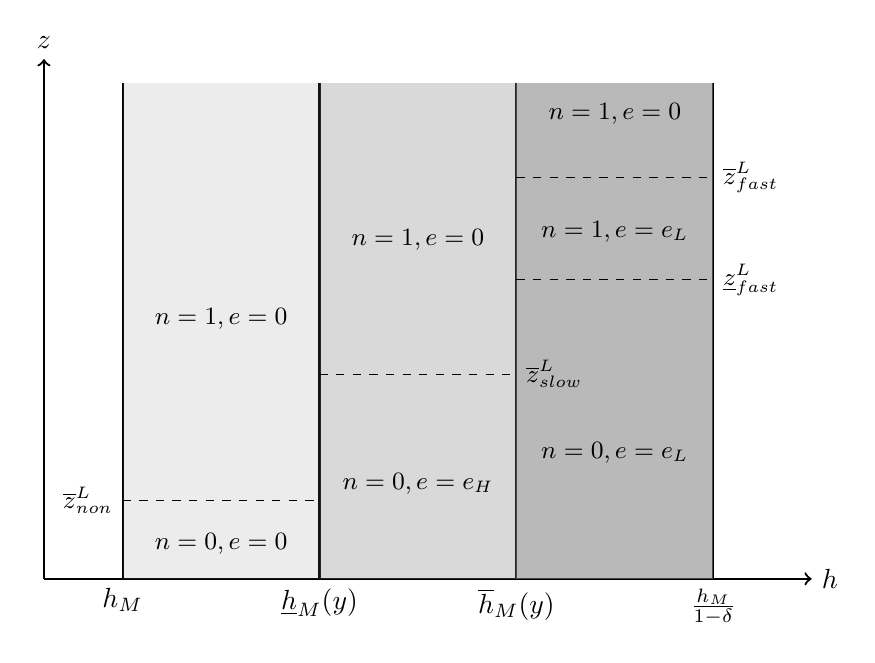
\begin{tikzpicture}[xscale=1.25]

% Decision rule conditional on a given y:
% x-axis: h in [h_M, h_M/(1-delta))
% y-axis: z

% Axes
\draw[thick,->] (-0.8,0) -- (7,0) node[right] {$h$};
\draw[thick,->] (-0.8,0) -- (-0.8,6.6) node[above] {$z$};

% h-range boundaries
\draw[thick] (0,0) -- (0,6.3);
\node[below] at (0,0) {$h_M$};
\draw[thick] (6,0) -- (6,6.3);
\node[below] at (6,0) {$\frac{h_M}{1-\delta}$};


% Learner-type cutoffs in h conditional on y (schematic placement)
\draw[thick] (2,0) -- (2,6.3);
\draw[thick] (4,0) -- (4,6.3);
\node[below] at (2,0) {$\underline{h}_M(y)$};
\node[below] at (4,0) {$\overline{h}_M(y)$};

% Shade learner-type regions (conditional on y)
\fill[gray, opacity=0.15] (0,0) rectangle (2,6.3); % non-learners
\fill[gray, opacity=0.30] (2,0) rectangle (4,6.3); % slow learners
\fill[gray, opacity=0.55] (4,0) rectangle (6,6.3); % fast learners

% z cutoffs (schematic heights)
\def\zNon{1.0}
\def\zSlow{2.6}
\def\zFastL{3.8}
\def\zFastU{5.1}

% Non-learner cutoff
\draw[dashed] (0,\zNon) -- (2,\zNon);
\node[left] at (0,\zNon) {\small $\overline{z}^L_{non}$};

% Slow-learner cutoff
\draw[dashed] (2,\zSlow) -- (4,\zSlow);
\node[right] at (4,\zSlow) {\small $\overline{z}^L_{slow}$};

% Fast-learner cutoffs
\draw[dashed] (4,\zFastL) -- (6,\zFastL);
\draw[dashed] (4,\zFastU) -- (6,\zFastU);
\node[right] at (6,\zFastL) {\small $\underline{z}^L_{fast}$};
\node[right] at (6,\zFastU) {\small $\overline{z}^L_{fast}$};

% Decision labels inside regions
% Non-learners
\node at (1,0.45) {\small $n=0,e=0$};
\node at (1,3.3) {\small $n=1,e=0$};

% Slow learners
\node at (3,1.2) {\small $n=0,e=e_H$};
\node at (3,4.3) {\small $n=1,e=0$};

% Fast learners
\node at (5,1.6) {\small $n=0,e=e_L$};
\node at (5,4.4) {\small $n=1,e=e_L$};
\node at (5,5.9) {\small $n=1,e=0$};

\end{tikzpicture}

\end{document}

\caption{Decision Rule Diagram for $h_M \leq h<h_M(1-\delta)^{-1}$}
\begin{flushleft}
\footnotesize{The human capital $h$ changes along the horizontal line and the idiosyncratic productivity $z$ changes along the vertical line. The two diagonal lines, $\overline{z}_M(h)$ and $\underline{z}_M(h)$, separate the state space into three areas: the unshaded area represents the non-learners, the lightly-shaded area represents the slow learners, and the darkly-shaded  area represents the fast learners. The areas are divided by four dashed horizontal lines associated with cutoffs $\overline{z}^L_{non}$, $\overline{z}^L_{slow}$, $\underline{z}^L_{fast}$, and $\overline{z}^L_{fast}$ that are functions of capital holding $a$.} 
\end{flushleft}
    
\label{fig:rule-diagram}
\end{figure}

\paragraph{Decision rule diagram for households:}Figure \ref{fig:rule-diagram} illustrates the decision rule $(n,e)$ as a function of states $(z,h,a)$ for households with $h_M \leq h<h_M\frac{1}{1-\delta}$. The human capital $h$ changes along the horizontal line and the idiosyncratic productivity $z$ changes along the vertical line. The two diagonal lines, $\overline{z}_M(h)$ and $\underline{z}_M(h)$ defined in (\ref{eq:zm}), separate the state space into three areas: the unshaded area represents the non-learners, the lightly-shaded area represents the slow learners, and the darkly-shaded area represents the fast learners. The areas are divided by four dashed horizontal lines associated with cutoffs $\overline{z}^L_{non}(a)$, $\overline{z}^L_{slow}(a)$, $\underline{z}^L_{fast}(a)$, and $\overline{z}^L_{fast}(a)$ that are functions of capital holding $a$ and defined in (\ref{eq:z-non}), (\ref{eq:z-slow}), (\ref{eq:z-fast-lower}), and (\ref{eq:z-fast-upper}).

This decision rule diagram is representative for households with other levels of human capital. For households with $h<h_M$, $\overline{z}_M(h)$ and $\underline{z}_M(h)$ continue to be the boundaries that separate non-learners, slow learners and fast learners, but the four cutoffs are $\overline{z}^L_{non}\frac{1}{1-\lambda}$, $\overline{z}^L_{slow}\frac{1}{1-\lambda}$, $\underline{z}^L_{fast}\frac{1}{1-\lambda}$, and $\overline{z}^L_{fast}\frac{1}{1-\lambda}$.

For households with $h_M\frac{1}{1-\delta} \leq h<h_H\frac{1}{1-\delta}$, the boundaries for state space division change to $\overline{z}_H(h)$ and $\underline{z}_H(h)$:
\begin{equation}\label{eq:zh}
    \underline{z}_H(h):=\frac{h_H-(1-\delta)h}{e_H}; \overline{z}_H(h):=\frac{h_H-(1-\delta)h}{e_L} 
\end{equation}
If $h_M\frac{1}{1-\delta} \leq h<h_H$, the four cutoffs for households are:\footnote{Appendix provides parameter restrictions for $\overline{z}^M_{fast}(a)>\underline{z}^M_{fast}(a)$.}
\begin{align}
\overline{z}^M_{non}(a)&:=\frac{(\exp(\frac{\chi_n}{1+\beta})-1)[(1+r)a+\frac{w'z'}{1+r'}]}{w}  \label{eq:z-non-M} \\
\overline{z}^M_{slow}(a)&:=\frac{(\exp(\frac{\chi_n-\chi_e e_H}{1+\beta})-1)[(1+r)a+\frac{w'z'(1+\lambda)}{1+r'}]+\lambda\frac{w'z'}{1+r'}}{w} \label{eq:z-slow-M} \\
\underline{z}^M_{fast}(a)&:=\frac{(\exp(\frac{\chi_n}{1+\beta})-1)[(1+r)a+\frac{w'z'(1+\lambda)}{1+r'}]}{w} \label{eq:z-fast-lower-M} \\
\overline{z}^M_{fast}(a)&:=\frac{\left\{\lambda\left[\exp(\frac{\chi_e e_L}{1+\beta})-1\right]^{-1}-1\right\}\frac{w'z'}{1+r'}-(1+r)a}{w}  \label{eq:z-fast-upper_M} 
\end{align}
If $h_H \leq h<h_H\frac{1}{1-\delta}$, the cutoffs are $\overline{z}^M_{non}\frac{1}{1+\lambda}$, $\overline{z}^M_{slow}\frac{1}{1+\lambda}$, $\underline{z}^M_{fast}\frac{1}{1+\lambda}$, and $\overline{z}^M_{fast}\frac{1}{1+\lambda}$.


All households with $h \geq h_H\frac{1}{1-\delta}$ are non-learners because their current human capital is enough for employment in the high sector next period even without any human capital investment. The only relevant cutoff for them is $\overline{z}^H_{non}(a)\frac{1}{1+\lambda}$ where
\begin{equation}
    \overline{z}^H_{non}(a):=\frac{(\exp(\frac{\chi_n}{1+\beta})-1)[(1+r)a+\frac{w'z'(1+\lambda)}{1+r'}]}{w}  \label{eq:z-non-H} 
\end{equation}



\subsection{Comparative Statics}
The decision rules derived in the previous section imply that the fast learners invest in human capital if $z<\overline{z}_{fast}(h,a)$ and the slow learner invest in human capital if $z<\overline{z}_{slow}(h,a)$. The close form expressions of the cutoffs allow us to compare human capital investment between groups of households with different levels of human capital and physical capital.

\paragraph{Effect of human capital $h$ on human capital investment:} 

\begin{lemma}\label{lem:h_on_e}
    Both the fast learners and the slow learners with $h<\frac{h_M}{1-\delta}$ invest more in human capital than their counterparts with $h>\frac{h_M}{1-\delta}$:
    \begin{align*}
        \frac{\overline{z}^L_{fast}}{1-\lambda} &> \overline{z}^M_{fast} \text{ ; }  \overline{z}^L_{fast}> \frac{\overline{z}^M_{fast}}{1+\lambda}\\
        \frac{\overline{z}^L_{slow}}{1-\lambda} &> \overline{z}^M_{slow} \text{ ; }  \overline{z}^L_{slow}> \frac{\overline{z}^M_{slow}}{1+\lambda}
    \end{align*}
    
\end{lemma}

\begin{figure}
    \centering
    
\documentclass{standalone}
\usepackage{tikz}
\usetikzlibrary{patterns}
\begin{document}
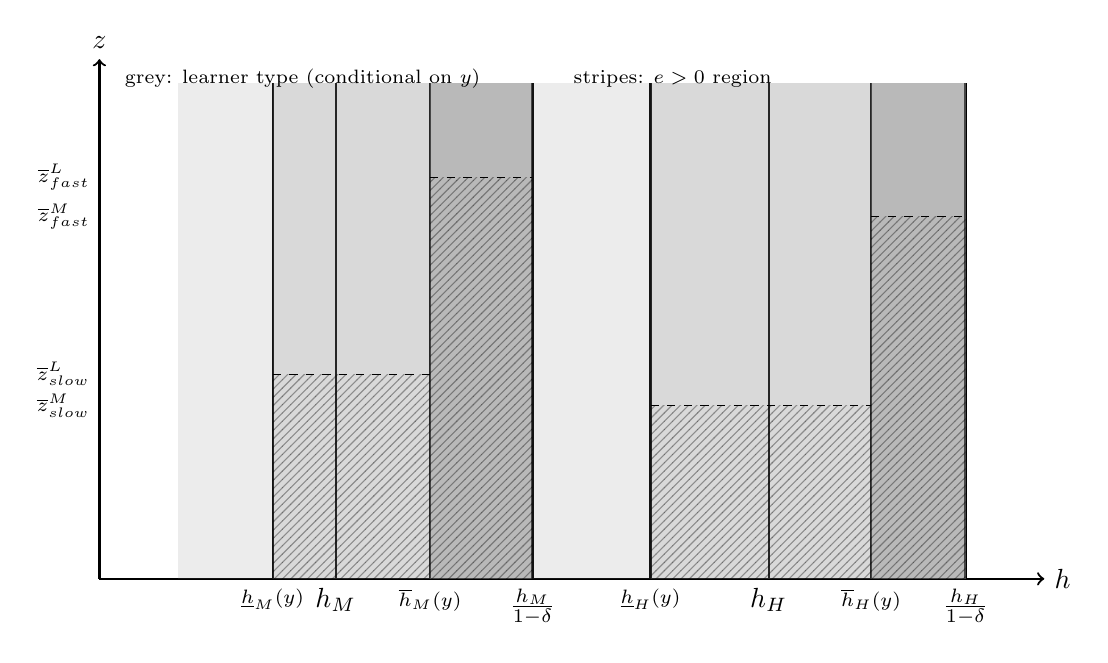
\begin{tikzpicture}

% Axes
\draw[thick,->] (-1,0) -- (11,0) node[right] {$h$};
\draw[thick,->] (-1,0) -- (-1,6.6) node[above] {$z$};

% Key h cutoffs
\draw[thick] (2,0) -- (2,6.3);
\node[below] at (2,0) {$h_M$};
\draw[thick] (4.5,0) -- (4.5,6.3);
\node[below] at (4.5,0) {$\frac{h_M}{1-\delta}$};
\draw[thick] (7.5,0) -- (7.5,6.3);
\node[below] at (7.5,0) {$h_H$};
\draw[thick] (10,0) -- (10,6.3);
\node[below] at (10,0) {$\frac{h_H}{1-\delta}$};

% h-cutoffs conditional on y (schematic placement, labels carry the economics)
% Relative to h_M
\draw[thick] (1.2,0) -- (1.2,6.3);
\draw[thick] (3.2,0) -- (3.2,6.3);
\node[below] at (1.2,0) {\scriptsize $\underline{h}_M(y)$};
\node[below] at (3.2,0) {\scriptsize $\overline{h}_M(y)$};
% Relative to h_H
\draw[thick] (6.0,0) -- (6.0,6.3);
\draw[thick] (8.8,0) -- (8.8,6.3);
\node[below] at (6.0,0) {\scriptsize $\underline{h}_H(y)$};
\node[below] at (8.8,0) {\scriptsize $\overline{h}_H(y)$};

% Grey shading: learner types (conditional on y), by h
% Left block (threshold h_M): [0,4.5]
\fill[gray, opacity=0.15] (0,0) rectangle (1.2,6.3);  % non-learners
\fill[gray, opacity=0.30] (1.2,0) rectangle (3.2,6.3); % slow learners
\fill[gray, opacity=0.55] (3.2,0) rectangle (4.5,6.3); % fast learners
% Right block (threshold h_H): [4.5,10]
\fill[gray, opacity=0.15] (4.5,0) rectangle (6.0,6.3);  % non-learners
\fill[gray, opacity=0.30] (6.0,0) rectangle (8.8,6.3);  % slow learners
\fill[gray, opacity=0.55] (8.8,0) rectangle (10,6.3);   % fast learners

% Stripes: region where e>0 (schematic, uses z cutoffs)
% Define schematic z cutoffs
\def\zSlowL{2.6}   % \overline{z}^L_{slow}
\def\zFastL{5.1}   % \overline{z}^L_{fast}
\def\zSlowM{2.2}   % \overline{z}^M_{slow}
\def\zFastM{4.6}   % \overline{z}^M_{fast}

% Left block: investment for slow learners (e_H) when z is low
\fill[pattern=north east lines, pattern color=black, opacity=0.35]
  (1.2,0) rectangle (3.2,\zSlowL);
% Left block: investment for fast learners (e_L) when z is below \overline{z}^L_{fast}
\fill[pattern=north east lines, pattern color=black, opacity=0.35]
  (3.2,0) rectangle (4.5,\zFastL);

% Right block: investment for slow learners (e_H) when z is low
\fill[pattern=north east lines, pattern color=black, opacity=0.35]
  (6.0,0) rectangle (8.8,\zSlowM);
% Right block: investment for fast learners (e_L) when z is low
\fill[pattern=north east lines, pattern color=black, opacity=0.35]
  (8.8,0) rectangle (10,\zFastM);

% Dashed horizontal cutoff lines (labels)
\draw[dashed] (1.2,\zSlowL) -- (3.2,\zSlowL);
\node[left] at (-1,\zSlowL) {\scriptsize $\overline{z}^L_{slow}$};
\draw[dashed] (3.2,\zFastL) -- (4.5,\zFastL);
\node[left] at (-1,\zFastL) {\scriptsize $\overline{z}^L_{fast}$};
\draw[dashed] (6.0,\zSlowM) -- (8.8,\zSlowM);
\node[left] at (-1,\zSlowM) {\scriptsize $\overline{z}^M_{slow}$};
\draw[dashed] (8.8,\zFastM) -- (10,\zFastM);
\node[left] at (-1,\zFastM) {\scriptsize $\overline{z}^M_{fast}$};

% Legend (minimal)
\node[anchor=west] at (-0.8,6.35) {\scriptsize grey: learner type (conditional on $y$)};
\node[anchor=west] at (4.9,6.35) {\scriptsize stripes: $e>0$ region};

\end{tikzpicture}
\end{document}


\caption{State Space for Human Capital Investment}
\begin{flushleft}
\footnotesize{The darkly-shaded striped areas indicate the state space for human capital investment equal to $e_L$ by the fast learners. The lightly-shaded striped areas indicate the state space for human capital investment equal to $e_H$ by the slow learners.} 
\end{flushleft}
    
\label{fig:e-digram}
\end{figure}

Figure \ref{fig:e-digram} provides an illustration to this proposition. The striped areas indicate the state space for positive human capital investment. The darkly-shaded areas correspond to the fast learners. The lightly-shaded areas correspond to the slow learners. Let us take the slow learners as an example. Those with $h<\frac{h_M}{1-\delta}$ need to invest $e_H$ to either stay in or to move up to the middle sector next period. Those with $h>\frac{h_M}{1-\delta}$ need to invest $e_H$ to either stay in or to move up to the high sector. The most productive households does not invest in human capital because it requires giving up their labor earning. This productivity cutoff is lower for those with higher human capital, meaning that their investment in human capital is lower than those with lower human capital. 



\paragraph{Effect of physical capital $a$ on human capital investment:} 
\begin{lemma}\label{lem:a_on_e}
The fast learners with lower asset holding invest more in human capital:
\begin{equation*}
    \frac{\partial \overline{z}^L_{fast}(a)}{\partial a}<0 \text{ ; } \frac{\partial \overline{z}^M_{fast}(a)} {\partial a} <0
\end{equation*}
The slow learners with lower asset holding invest more in human capital if and only if $\chi_n<\chi_e e_H$:
\begin{equation*}
    \frac{\partial \overline{z}^L_{slow}(a)}{\partial a}<0 \text{ and } \frac{\partial \overline{z}^M_{slow}(a)}{\partial a}<0 \text{ iff } \chi_n<\chi_e e_H
\end{equation*}
\end{lemma}
    


\subsection{The Effects of an Anticipated Period-2 AI Shock}
Suppose that an AI shock is anticipated to occur in period 2 and to increase the labor productivity for the low sector and the high sector but not the middle sector. The effect of AI shock on the sectoral productivity is captured by $\gamma$ with $0<\gamma<1$:
\begin{equation}
    \label{eq:xAI}
x(h')=\left \{ 
\begin{array}{cl}
1-\lambda + \gamma \lambda & \text{low sector if }h'<h_{M} \\ 
1 & \text{middle sector if }h_{M}<h'<h_{H} \\ 
1+\lambda + \gamma \lambda & \text{high sector if }h'>h_{H}%
\end{array}%
\right. 
\end{equation}
In other words, the AI shock increases average labor productivity, reduces the earnings premium for the middle sector, and enlarges the earnings premium for the high sector relative to the middle sector.

\paragraph{The non-learners:} The AI shock increases the labor income of households who work in the low sector or the high sector in period 2, i.e, those with $h<h_M\frac{1}{1-\delta}$ or $h>h_H\frac{1}{1-\delta}$. The positive income effect makes them work less in period 1 so that $\overline{z}^L_{non}(a)$ and $\overline{z}^H_{non}(a)$ increases in $\gamma$:
\begin{equation*}
    \overline{z}^i_{non}(a;\gamma)=\overline{z}^i_{non}(a;\gamma=0) + \gamma \lambda  \frac{w'z'}{w(1+r')}\left[\exp(\frac{\chi_n}{1+\beta})-1\right] \text{ for } i=L,H
\end{equation*}


\paragraph{The slow learners:} The AI shock reduces the incentive to work in the middle sector in period 2, i.e., $\overline{z}^L_{slow}(a)$ is decreasing and $\overline{z}^M_{slow}(a)$ is increasing in $\gamma$:
\begin{align*}
    \overline{z}^L_{slow}(a;\gamma)&= \overline{z}^L_{slow}(a;\gamma=0) - \gamma \lambda  \frac{w'z'}{w(1+r')}\\
    \overline{z}^M_{slow}(a;\gamma)&=\overline{z}^M_{slow}(a;\gamma=0) + \gamma \lambda \frac{w'z'}{w(1+r')}\exp(\frac{\chi_n-\chi_e e_H}{1+\beta})
\end{align*}
Therefore, those with $h<h_M\frac{1}{1-\delta}$ invest less human capital and work more in period 1 and those with $h>h_M\frac{1}{1-\delta}$ invest more human capital and work less.

\paragraph{The fast learners:} Similar to the slow learners, the AI shock reduces households' incentive to work in the middle sector in period 2. As a result, human capital investment is lower for those with $h<h_M\frac{1}{1-\delta}$, and is higher for those with $h>h_M\frac{1}{1-\delta}$. The effects of AI shock $\gamma$ on the cutoff governing human capital investment are:
\begin{align*}
    \overline{z}^L_{fast}(a;\gamma)&= \overline{z}^L_{fast}(a;\gamma=0) - \gamma \lambda \frac{w'z'}{w(1+r')}\frac{\exp(\frac{\chi_e e_L}{1+\beta})}{\exp(\frac{\chi_e e_L}{1+\beta})-1} \\
    \overline{z}^M_{fast}(a;\gamma)&= \overline{z}^M_{fast}(a;\gamma=0) + \gamma \lambda \frac{w'z'}{w(1+r')}\frac{1}{\exp(\frac{\chi_e e_L}{1+\beta})-1} 
\end{align*}
Conditional on the human capital investment being $e_L$, the fast learners' labor supply decision is affected by the AI shock via the future earning increase if the households will work in the high sector in period 2. That is, those with $h>h_M\frac{1}{1-\delta}$ work less in period 1, i.e., $\underline{z}^L_{fast}$ increases in $\gamma$:
\begin{equation*}
    \underline{z}^M_{fast}(a;\gamma)=\underline{z}^M_{fast}(a;\gamma=0) + \gamma \lambda \frac{w'z'}{w(1+r')}\left[\exp(\frac{\chi_n}{1+\beta})-1\right]
\end{equation*}

\subsubsection{AI effect on human capital inequality}
Recall from Lemma \ref{lem:h_on_e} that, without the AI shock, households with low $h$ invest more in human capital than households with high $h$. The analysis above shows that the AI shock discourages human capital investment for those with low $h$ but encourages it for those with high $h$. Therefore, a small AI shock reduces human capital investment disparity between groups with different levels of $h$, and a large AI shock could lead to a reversal in the comparison, making households with high $h$ invest more in human capital than households with low $h$. The human capital distribution will be more unequal due to the AI shock. 
\begin{proposition}
    AI shock increases human capital inequality.
\end{proposition}

\subsubsection{AI effect on consumption inequality}
According to the optimal consumption rule in (\ref{eq:c'}) and (\ref{eq:c}), consumption is proportional to the present value of household incomes in two periods. The AI shock increases the period-2 labor income of the low and high sectors, and in turn increases the consumption of households who would have worked in the low or the high sector in period 2 without the AI shock. 

For households with $h<h_M\frac{1}{1-\delta}$, the affected groups are those whose human capital investment would be zero without the AI shock. In Figure \ref{fig:e-digram}, they are the unstriped areas to the left of the vertical line $\frac{h_M}{1-\delta}$. Within the fast learners, it is the households with higher current $z$ that are affected by the AI shock and have their consumption increased. Since higher current $z$ is associated with a higher consumption, the AI shock increases the consumption inequality within the fast learners. The same argument applies to the slow learners. 

By contrast, the affected groups for households with $h_M\frac{1}{1-\delta}<h<h_H\frac{1}{1-\delta}$ are those whose human capital investment would be positive without the AI shock. In Figure \ref{fig:e-digram}, they are the striped areas to the right of the vertical line $\frac{h_M}{1-\delta}$. Within the fast learners, the AI shock increases the consumption of the households with lower current $z$, therefore reducing the consumption inequality. The same argument applies to the slow learners. 
\begin{proposition}
    AI shock increases consumption inequality within the fast (slow) learners of low human capital, $h<h_M\frac{1}{1-\delta}$. AI shock reduces consumption inequality within the fast (slow) learners of high human capital, $h>h_M\frac{1}{1-\delta}$.
\end{proposition}

For the non-learners, the AI shock only affects those with $h_M\frac{1}{1-\delta}<h<h_H\frac{1}{1-\delta}$, moving their consumption closer to those with lower $h$ and lower consumption, but away from those with higher $h$ and higher consumption. 

\subsection{The Effects of Uninsured Idiosyncratic Risk}
We now reintroduce the idiosyncratic risk to households in period 1 by assuming that $z'$ follows a log-normal distribution with mean $\overline{z}'$ and variance $\sigma^2_z$. 

Our previous analysis without uncertainty is a special case with $\sigma^2_z=0$. The effects of uninsured idiosyncratic risk can be thought as how households' decisions change when the distribution of $z'$ undergoes a mean-preserving spread in the sense of second-order stochastic dominance.

From a consumption-saving perspective, the uncertain $z'$ is associated with future labor income risk. It is well understood in the literature that idiosyncratic future income risk raises the expected marginal utility of future consumption for households with log utility and makes them save more. In our model, households can also supply more labor to mitigate the effect of idiosyncratic income risk on the marginal utility of consumption. 

From the perspective of human capital investment, the uncertain $z'$ is associated with risk in the return to human capital. Conditional on working, households' income increases with $z'$: $c'=(1+r')a'+w'x(h')z'$. $\ln(c')$ is increasing and concave in $z'$, and a higher $x(h')$ increases the concavity.\footnote{The marginal effect of $z'$ on $\ln(c')$ is 
\begin{equation*}
    \frac{\partial\ln(c')}{\partial z'}=\frac{w'x(h')}{(1+r')a'+w'x(h')z'} > 0
\end{equation*}
The second derivative is 
\begin{equation*}
    \frac{\partial^2\ln(c')}{(\partial z')^2}=-\left[\frac{w'x(h')}{(1+r')a'+w'x(h')z'}\right]^2 <0
\end{equation*}
and is more negative if $x(h')$ is higher.} Consider two levels of $h'$, $\overline{h'}>\underline{h'}$, a mean-preserving spread of $z'$ distribution reduces the expected utility at both levels of $h'$ but the reduction is larger for the higher level $\overline{h'}$. Hence, the expected utility gain of moving from $\underline{h'}$ to $\overline{h'}$ is smaller due to the idiosyncratic risk. Human capital investment is discouraged.

Taking into account endogenous labor supply reinforces the discouragement of human capital investment by the idiosyncratic risk. Recall from Section \ref{sec:period2} that households with $z'$ lower than a cutoff do not work. The endogenous labor supply therefore provides insurance against the lower tail risk of the idiosyncratic $z'$. Moreover, the cutoff in $z'$ is lower for those with higher human capital $h'$. This makes households with higher $h'$ more exposed to the lower tail risk than those with lower $h'$, further reducing the gain of human capital investment.


\begin{proposition}
    The uninsured idiosyncratic risk in $z'$ makes households in period 1 save more, work more and invest less in human capital.
\end{proposition}

\paragraph{Limitations to the two-period model:} In the two-period model, we take the period-1 asset holding as exogenous. In the full model, the idiosyncratic risk increases households saving and leads to more asset holding. According to Lemma \ref{lem:a_on_e}, more asset holding reduces human capital investment for the fast learners and reduces human capital investment for the slow learners if and only if $\chi_n<\chi_e e_H$.


\section{A Quantitative Model \protect\label{sec:quant_model}}

We now solve the full dynamic model with infinite horizon, endogenous asset accumulation, and general equilibrium. 
We calibrate the model to reflect key features of the U.S. economy,
capturing reasonable household heterogeneity. 

\subsection{Calibration \protect\label{sec:calib}}

We calibrate the model to match the U.S. economy. For several preference
parameters, we adopt values commonly used in the literature. Other
parameters are calibrated to align with targeted moments. The model
operates on an annual time period. Table \ref{tbl:para} summarizes
the parameter values used in the benchmark model.

\begin{table}
\noindent{}%
\noindent\begin{minipage}[t]{1\columnwidth}%
\begin{center}
\caption{\protect\label{tbl:para}Parameters for the Calibration}

\begin{tabular}{crrll}
\toprule 
~Parameter  & Value  &  & Description  & Target or Reference\tabularnewline
\midrule 
$\beta$  & 0.91795 &  & Time discount factor  & Annual interest rate\tabularnewline
$\rho_{z}$  & 0.94  &  & Persistence of $z$ shocks  & See text\tabularnewline
$\sigma_{z}$  & 0.287  &  & Standard deviation of $z$ shocks  & Earnings Gini\tabularnewline
$\underline{a}$  & 0  &  & Borrowing limit  & See text\tabularnewline
$\chi_{n}$  & 2.47  &  & Disutility from working  & Employment rate\tabularnewline
$\chi_{e}$  & 1.48  &  & Disutility from HC effort  & See text\tabularnewline
$\overline{n}$  & 1/3  &  & Hours worked  & Average hours worked\tabularnewline
$e_{H}$  & 1/3  &  & High level of effort  & Average hours worked\tabularnewline
$e_{L}$  & 1/6  &  & Low level of effort  & See text\tabularnewline
$h_{M}$  & 0.41  &  & Human capital cutoff for M  & See text\tabularnewline
$h_{H}$  & 0.96  &  & Human capital cutoff for H  & See text\tabularnewline
$\lambda$  & 0.2  &  & Skill premium  & Income Gini\tabularnewline
$\alpha$  & 0.36  &  & Capital income share  & Standard value\tabularnewline
$\delta$  & 0.1  &  & Capital depreciation rate  & Standard value\tabularnewline
\bottomrule
\end{tabular}
\par\end{center}%
\end{minipage}
\end{table}

The time discount factor, $\beta$, is calibrated to match an annual
interest rate of 4 percent. We set $\chi_{n}$ to replicate an 80
percent employment rate. We calibrate $\chi_{e}$ to match the fact
that around 30 percent of the population invests in human capital.
The borrowing limit, $\text{\underbar{\ensuremath{a}},}$ is set to
0. 

We calibrate parameters regarding labor productivity process as follows.
We assume that $x$ follows the AR(1) process in logs: $\log z'=\rho_{z}\log z+\epsilon_{z}$,
where $\epsilon_{z}\sim N(0,\sigma_{z}^{2})$. The shock process is
discretized using the Tauchen (1986) method, resulting in a transition
probability matrix with 9 grids. The persistence parameter $\rho_{z}=0.94$
is chosen based on estimates from the literature. The standard deviation
$\sigma_{z}$, is chosen to match the earnings Gini coefficient of 0.63.

We deviate from the two-period model by assuming that the labor supply is a discrete choice between 0 and $\overline{n}=1/3$. This change only rescales the two-period model without altering the trade-off facing the households. But such rescaling facilitates the interpretation that households are deciding whether to allocate one-third of their fixed time endowment to work. The high-level human capital accumulation
effort, $e_{H}$ is assumed to equal $\overline{n}.$ The low-level
effort, $e_{L}$ is set to half of $e_{H}$. The skill premium across
sectors, $\lambda,$ is set at 0.2 to match the income Gini coefficient.
Human capital cutoffs, $h_{M}$ and $h_{H}$, are set so that the population shares in low, middle, and high sectors are, respectively, 20, 40, and 40 percent. This population distribution roughly matches the fractions of U.S. workers in 2014 who are employed in routine manual occupations (low sector), routine cognitive and non-routine manual (middle sector), and non-routine cognitive (high sector) \cite{cortes_disappearing_2017}.


On the production side, we set the capital income share, $\alpha,$ to 0.36, and the depreciation rate, $\delta,$ to 0.1.

\begin{table}
\caption{\protect\label{tbl:moments}Key Moments}

\begin{centering}
\begin{tabular}{lccccrrrc}
\hline 
Moment  &  &  &  & Data  &  &  &  & Model\tabularnewline
\hline 
~~Employment rate  &  &  &  & 0.80  &  &  &  & 0.80\tabularnewline
~~Human capital investment ratio  &  &  &  & 0.29  &  &  &  & 0.29\tabularnewline
~~Gini coefficient for wealth  &  &  &  & 0.78  &  &  &  & 0.76\tabularnewline
~~Gini coefficient for earnings  &  &  &  & 0.63  &  &  &  & 0.62\tabularnewline
~~Gini coefficient for income  &  &  &  & 0.57  &  &  &  & 0.58\tabularnewline
\hline 
\end{tabular}
\par\end{centering}
\end{table}


\subsection{Key Moments: Data vs. Model}

In Table \ref{tbl:moments}, we present a comparison of
key moments between the model and the empirical data. The model does
an excellent job of replicating the 80\% employment rate observed
in the data. In this context, employment is defined as having positive
labor income in the given year, consistent with the common approach
used in the literature. According to \citet{OECD1998}, the share
of the population investing in human capital---those who are actively
engaged in skill acquisition or education---is approximately 30\%,
a figure well matched by the model\textquoteright s predictions. This
is an important metric because it reflects the model's capacity to
capture the dynamics of human capital formation, which plays a critical
role in shaping long-run earnings and income inequality. Additionally,
the model accurately captures the distribution of income and earnings,
aligning closely with observed data. This suggests that the model
effectively incorporates the key mechanisms driving labor market outcomes
and the corresponding distributional aspects of earnings. Although the model does not explicitly target the wealth Gini coefficient, it achieves a close match to the data: the empirical wealth Gini is 0.78, while the model produces a value of 0.76. This highlights the model’s ability to capture substantial wealth inequality in the economy.


\subsection{Steady-state Distribution}
Table \ref{tab:SSdistribution} presents the steady-state distribution of population, employment, and assets across sectors. The population shares are calibrated to 20\%, 40\%, and 40\% by adjusting the human capital thresholds that define sectors. The shares of employment and assets are endogenously determined by households' labor supply and savings decisions. Notably, the high sector accounts for 46\% of total employment—exceeding its population share—indicating that a disproportionate number of households choose to work in that sector. Asset holdings are even more skewed: the high sector holds 68\% of total assets, while the low sector holds only 8\%.  
 
% Table generated by Excel2LaTeX from sheet 'Sheet1'
\begin{table}[htbp]
\begin{centering}
\caption{Distribution of Population, Employment and Assets}
\begin{tabular}{lccc}
\toprule 
Sectors  & \multicolumn{1}{l}{Pop. Share (\%)} & \multicolumn{1}{l}{Emp. Share (\%)} & \multicolumn{1}{l}{Assets Share (\%)}\tabularnewline
\midrule 
Low  & 20.76 & 18.58 & 8.07\tabularnewline
Middle  & 38.87 & 35.35 & 23.92\tabularnewline
High  & 40.35 & 46.07 & 68.01\tabularnewline
\bottomrule
\end{tabular}\label{tab:SSdistribution}
\par\end{centering}
{\scriptsize Note: Human capital cutoffs, $h_{H}$ and $h_{M}$, determine
the population share across sectors. Employment share and assets share
are implied by households labor supply decisions and saving decisions. }{\scriptsize\par}
\end{table}


\section{AI's Impact on Human Capital Adjustments}
\begin{figure}
    \centering  
    \caption{Steady-state Human Capital Distribution}
    \includegraphics[width=0.9\linewidth]{figure_204040calib/h_dist.pdf}
    \label{fig:hc_dist}   
    \caption{Steady-state Human Capital Investment}
    \includegraphics[width=0.9\linewidth]{figure_204040calib/DR_h.pdf}
    \label{fig:hprime_h}    
    \caption{Transition Path for Human Capital Investment}
    \includegraphics[width=0.9\linewidth]{figure_204040calib/agg_HC.pdf}
    \label{fig:h_agg}
    
\end{figure}
We now introduce AI technology into the quantitative model, assuming that it will be implemented in 10 years and that households have full information about its arrival. We examine both the transition dynamics and the differences between the initial and new steady states. This framework allows us to analyze how the economy adjusts in anticipation of, and in response to, the adoption of AI.

The effect of AI on the sectorial productivity is modeled as in (\ref{eq:xAI}) with $\gamma=0.3$. That is, AI boosted the productivity of the low sector workers by 7.5\% and the productivity of the high sector workers by 5\%, leaving the middle sector intact. It captures the key idea that AI increases average labor productivity \parencites{Acemoglu2019a}, but reduces the earning premium for the middle sector, and enlarges the earning premium for the higher sector relative the middle sector. 



\subsection{Human Capital Adjustments}
Given the employment distribution in the initial steady state, AI is projected to increase the economy's labor productivity by 4\% on average, assuming households do not alter their decisions in response. However, changes in earning premiums incentivize households to adjust their human capital investments. 

\paragraph{Steady-state human capital distribution:}
Figure \ref{fig:hc_dist} illustrates how households reallocate across sectors in the new steady state relative to the initial one. The x-axis denotes the level of human capital, while the y-axis indicates the mass of households at each human capital level. The red vertical line marks the cutoff between the low and middle sectors, and the blue vertical line marks the cutoff between the middle and high sectors.

The gray shaded area shows the overlap between the two steady-state distributions. Within each sector, the distribution of households is skewed to the left, reflecting the tendency for human capital investment to be concentrated among those near the sectoral cutoffs. As shown in the decision rule diagram in Figure \ref{fig:e-digram}, some households seek to upgrade their skills, while others aim to remain in more skilled sectors. The blue shaded area highlights the mass of households who have exited the middle sector following the AI shock. The pink areas represent the additional mass of households in the new steady-state distribution, concentrated at the lower end of the low sector and the lower end of the high sector.

\paragraph{Steady-state human capital investment:}
This reallocation pattern reflects shifts in human capital investment incentives driven by AI’s impact on the skill premium. Figure \ref{fig:hprime_h} plots human capital investment decisions in the initial and new steady states across different human capital levels. Because both the productivity shock ($z$) and current asset holdings ($a$) influence human capital investment, the y-axis shows the weighted average of next-period human capital, where the weights reflect the steady-state distribution of households by productivity shock and wealth at each human capital level. 

The changes in decision rules before and after the AI shock are highlighted in the blue shaded area, where next-period human capital in the new steady state is lower than in the initial steady state, and in the pick shaded area, where it is higher. The most notable change is that the middle-sector households substantially intensify their human capital investment, aiming to transition into high-sector roles. In contrast, households in the low sector reduce their human capital investment, causing those who might have moved up to the middle sector to remain in the low sector or even drift further down to the very bottom of human capital distribution as shown in Figure \ref{fig:hc_dist}. 

Somewhat surprisingly, most high-sector workers in the new steady state decrease their human capital investment relative to the initial steady state. This is primarily a composition effect: as more households move from the middle-sector to the high sectors, the average asset holdings among high-sector households decline, making intensive human capital investment less affordable {\color{red} [note that this is not supported by the average asset in transition dynamics figure \ref{fig:tr_sector_k}]}. 

\paragraph{Transition path}
Figure \ref{fig:h_agg} reports the transition dynamics of aggregate human capital from the initial to the new steady state. The figure also displays its extensive margin (the share of households making positive human capital investments) and intensive margin (average human capital per household among those who invest).

As households reallocate from the middle sector to the low and high sectors, the net effect is a gradual decline in aggregate human capital along the transition path. This mirrors the steady-state change observed in Figure \ref{fig:hc_dist}, where the increased mass at the lower end of the low sector outweighs the increase in the high sector.

Additionally, human capital accumulation becomes increasingly concentrated among a smaller share of the population. The proportion of households making positive human capital investments steadily declines, ultimately stabilizing at a level 4\% lower than in the initial steady state. Meanwhile, the average human capital among those who invest rises, reaching a level 12\% higher than the initial steady state in the long run.\footnote{The only exception to those patterns occurs at period 10 when the positive effects of AI on sectoral productivity are realized.}



\subsection{Job Polarization}\label{sec:jobpolar}

An important implication of human capital adjustments to the AI shock is job polarization. 
Figure \ref{fig:tr_share} illustrate the transition paths of population shares and employment rates in each sector. Notably, the middle sector experiences a significant decline, with its population share decreasing by approximately 13\%. Additionally, employment within this sector plummets to a level 16\% lower than the initial steady state. In contrast, both the low and high sectors see increases in their population shares and employment rates. These dynamics indicate a reallocation of \emph{workers} from the middle sector to the low and high sectors following the introduction of AI.

\paragraph{Voluntary job polarization}
This worker reallocation aligns with the phenomenon of ``job polarization"\parencites{Goos2014}, where AI and automation technologies disproportionately replace tasks commonly performed by middle-skilled workers. However, our model introduces a complementary mechanism to the conventional understanding of this reallocation. Specifically, households in our model voluntarily exit the middle sector even before AI implementation by adjusting their human capital investments -- many middle-sector workers opt for non-employment to invest in skills that will better position
them for the post-AI labor market. To emphasize this key difference, our model deliberately abstracts from any direct negative effect of AI on middle-sector workers.

\paragraph{Employment flows more towards the low sector}

Another intriguing finding in our model is the more pronounced employment effect in the low sector compared to the high sector. In the new steady state, the employment rate in the low sector increases by 12\%, whereas in the high sector, it rises by only 0.5\%. This asymmetry in employment rate changes suggests an unbalanced reallocation of workers from the middle sector, with a greater flow toward the low sector.

This disparity arises from two key factors. First, AI enhances the productivity of low-sector workers by 7.5\% and high-sector workers by 5\%. However, this productivity differential alone does not fully account for the significant asymmetry. The second factor is the variation in labor supply elasticity across sectors. Compared to the high sector, the low sector exhibits higher labor supply elasticity, meaning that the same change in labor earnings triggers larger labor supply responses. This is because households in the low sector have lower consumption levels, making their marginal utility of consumption more sensitive to changes in their budget. Consequently, a greater proportion of households in the low sector are at the margin between employment and non-employment \citep{Chang2006}.


\begin{figure}
    \begin{centering}
    \caption{Sectoral Population and Employment Transition}
    \includegraphics[width=1\linewidth]{figure_204040calib/share}
    \label{fig:tr_share}
    \end{centering}\par
    {\scriptsize Note: The transition paths within each sector. The x-axis represents years, and the y-axis shows the percentage (or percentage point) deviation from the initial steady state. AI introduction is assumed to occur in period 10. “Pop. Share” denotes the population share within each sector. “Employment" is the percentage of households who are employed in each sector.}{\scriptsize\par}
\end{figure}







\section{The Aggregate and Distributional Effects of AI}
The aggregate and distributional effects of AI are shaped by both its direct impact on sectoral productivity and the endogenous response of human capital accumulation. By altering sectoral productivity, AI changes labor earnings, which in turn influences labor supply decisions and savings through income effects. Consequently, AI directly affects the supply of labor and capital, generating aggregate economic responses. Because AI’s productivity effects are heterogeneous across sectors, its impact is inherently distributional.

These sectoral differences also induce human capital adjustments, as households reallocate across sectors in response to changing incentives. This reallocation not only shifts the distribution of labor productivity and aggregate productivity, but also directly shapes distributional outcomes, as households’ relative positions in the income and asset distributions are altered by their movement across sectors.

In this section, we examine the importance of endogenous human capital adjustment in shaping both the transitional and long-run effects of AI. To do so, we compare the benchmark economy -- where households endogenously adjust their human capital -- with an alternative scenario in which households are held fixed at their initial steady-state human capital during the AI transition (“No HC model”). In both cases, households make endogenous decisions about consumption, savings, and labor supply. 

By contrasting the transition dynamics across these two economies, we can disentangle the direct and indirect effects of AI. The transition path in the No-HC-model isolates the direct impact of AI on aggregate and distributional outcomes, as it abstracts from any human capital adjustments. The difference in outcomes between the benchmark and the No-HC-model then reveals the indirect effects of AI that operate through households’ adjustments in human capital. This decomposition allows us to assess the relative importance of human capital dynamics in driving both the aggregate and distributional consequences of AI.


\subsection{Aggregate Implications}\label{sec:result}

\begin{figure}
\begin{centering}
\caption{\protect\label{fig:no_hc_1}Transition Path of Aggregate Variables:
Benchmark vs. No HC Models.}
\includegraphics[width=0.9\linewidth]{figure_204040calib/nohc_agg.pdf}
\par\end{centering}


{\scriptsize Note:  The transition paths of aggregate variables: benchmark vs. No HC models. The x-axis represents years, and the y-axis shows the percentage deviation from the initial steady state. AI introduction is assumed to occur in period 10. The No HC model is an economy in which workers maintain their initial steady-state level of human capital throughout the AI implementation until the new steady state is reached. }{\scriptsize\par}
\end{figure}

Figure \ref{fig:no_hc_1} shows the transition paths of key macroeconomic variables—output, consumption, investment, and employment—as well as factor prices, including the wage rate and capital return. The blue solid lines depict results from the benchmark model with endogenous human capital adjustment, while the black dashed lines represent the No-HC model in which human capital is held fixed.

\subsubsection{AI's direct impacts}

The No-HC-model isolates the direct effects of AI. In the long run, the introduction of AI leads to higher output, consumption, investment, and employment. However, in anticipation of AI (prior to period 10), output and investment decline, while consumption and employment remain stable.

Before the implementation of AI, sectoral productivity is unchanged; the only difference is households’ awareness of future increases in productivity in the low and high sectors beginning in period 10. This anticipation raises households’ expected lifetime income, prompting them to save less and consume more ahead of the actual productivity gains. As a result, aggregate capital stock falls, which lowers output and reduces the marginal product of labor while raising the marginal product of capital. Employment remains largely unchanged in this period, as sectoral productivity has not yet shifted.

Following the AI shock, sectoral productivity in the low and high sectors rises, boosting labor income, employment, and output in these sectors. Because productivity gains are labor-augmenting, the supply of efficient labor units rises sharply, causing wages to decline and capital returns to increase. Employment and investment both adjust to dampen these factor price changes. In the new steady state, the wage rate is slightly below its initial level, while the return to capital is marginally higher.

\subsubsection{AI's indirect impacts via endogenous human capital adjustments}

The difference between the No-HC model and the benchmark model captures the indirect effects of AI operating through endogenous human capital adjustments. Among all macroeconomic variables, this indirect effect is most pronounced for employment.

In anticipation of AI, employment declines as some households temporarily exit the labor market to invest in human capital and prepare for the post-AI economy.\footnote{Empirical studies, such as \citet{Lerch2021} and \citet{Faber2022}, support the short-term adverse effects of AI adoption on labor markets.} During this period, labor productivity remains unchanged, so the decline in employment directly translates to a reduction in output. Consistent with standard consumption-smoothing behavior, this reduction is mainly absorbed by lower investment. Meanwhile, the drop in employment mitigates the direct effects of AI on both wages and capital returns prior to the AI implementation.

After AI is introduced, employment rebounds as sectoral productivity increases. However, continued human capital investment by middle-sector households keeps employment lower than in the No-HC model, resulting in an almost neutral long-run effect of AI on employment. Despite this, output, consumption, and investment are all higher in the benchmark model because human capital adjustments reallocate more labor to the low and high sectors, thereby better capturing the productivity gains from AI.

This reallocation also reverses the steady-state comparison of factor prices: endogenous human capital adjustment transforms the negative direct effect of AI on the wage rate into a positive net effect, and the positive direct effect on capital returns into a negative net effect.


\subsection{Distributional Implications}

The findings above underscore the importance of accounting for human capital adjustments when assessing the aggregate impact of AI, as households actively adapt to a rapidly evolving labor market. When it comes to economic inequality, endogenously adjusting human capital plays an even more significant role.

Figure \ref{fig:no_hc_gini} shows the transition paths of Gini coefficients for earnings (labor income), total income (capital and labor income), consumption, wealth (asset holdings), and human capital. The black dashed lines represent results from the No-HC model, capturing the direct impact of AI without human capital adjustment. In contrast, the blue solid lines reflect the benchmark model, where human capital responds endogenously to both anticipated and realized changes in the skill premium induced by AI.

\subsubsection{Income, earnings, and consumption inequalities}
The comparison of transition paths between the No-HC model and the benchmark model reveals that endogenous human capital adjustments fundamentally alter the impact of AI on income, earnings, and consumption inequalities.

\paragraph{AI's direct impacts:} Without any human capital adjustments, AI's impact on inequalities is primarily driven by productivity gains in the low and high sectors -- 7.5\% and 5\%, respectively. As a result, there is little direct impact on income and earnings Gini coefficients in anticipation of AI before period 10. After AI is implemented, both income and earnings inequality decline: higher labor productivity raises earnings in the low sector, while wage declines in the middle sector compress the distribution. Consumption inequality remains largely unchanged throughout the transition.

\paragraph{Effects of AI-induced human capital adjustments:}
Allowing human capital to adjust endogenously, however, leads to pronounced job polarization, as shown in Section \ref{sec:jobpolar}. Households who would have qualified for middle-sector jobs now transition to either the low or high sector. Those moving to the low sector see reduced labor earnings, while those shifting to the high sector enjoy increased earnings. This polarization drives up earnings and income inequality, both before and after AI is implemented. As income disparities widen, consumption inequality also increases.



% This rise in inequality can
% be explained by the interactions among labor market dynamics, human
% capital accumulation, precautionary savings, and the differential
% impacts of AI on various sectors.

\begin{figure}
\begin{centering}
\caption{\protect\label{fig:no_hc_gini}Transition Path of Inequality Measures:
Benchmark vs. No HC Models.}
\par
\includegraphics[width=0.95\linewidth]{figure_204040calib/nohc_gini.pdf}
\par\end{centering}
{\scriptsize Note:  The transition paths of inequality measures: benchmark vs. No HC models. The x-axis represents years, and the y-axis shows the percentage deviation from the initial steady state. AI introduction is assumed to occur in period 10. The No HC model is an economy in which workers maintain their initial steady-state level of human capital throughout the AI implementation until the new steady state is reached.}{\scriptsize\par}


\end{figure}

\subsubsection{Wealth inequality} 

In stark contrast to the effects on income and earnings inequality, allowing for endogenous human capital adjustment actually mitigates the negative direct impact of AI on wealth inequality. While AI’s direct effect would otherwise widen disparities, human capital responses help dampen the increase in wealth inequality, underscoring the stabilizing role of human capital adjustments in the wealth distribution.

To disentangle the direct and indirect effects of AI on wealth inequality, Figure \ref{fig:tr_sector_k} presents the sectoral transition paths for asset holdings, while Figure \ref{fig:aprime_h} compares steady-state asset investment decisions across different human capital levels.
\begin{figure}
\begin{centering}

    \caption{\protect\label{fig:tr_sector_k}Sectoral Asset-holding Transition}
\includegraphics[width=0.9\linewidth]{figure_204040calib/nohc_asset.pdf}
\par\end{centering}

{\scriptsize Note: The transition paths of average capital within each sector. The x-axis represents years, and the y-axis shows the percentage deviation from the initial steady state. AI introduction is assumed to occur in period 10. “Average Capital” denotes the physical assets per household in each sector. }{\scriptsize\par}
\centering
\caption{Steady-state Asset Investment}
    \includegraphics[width=0.9\linewidth]{figure_204040calib/DR_a.pdf}    
    \label{fig:aprime_h}    
 
\end{figure}

{\color{red} [Add a figure that compares the steady-state asset investment in the No-HC-model (a counterpart of Figure \ref{fig:aprime_h}).]}

\paragraph{AI's direct impacts:} We first focus on the black dashed lines in Figure \ref{fig:tr_sector_k}. Without households reallocation across sectors, total assets and average asset holdings follow similar patterns. In both the low and high sectors, households reduce their savings in anticipation of AI, expecting higher lifetime labor income. After AI is implemented at period 10, their savings increase alongside rising labor incomes. In contrast, households in the middle sector, anticipating a negative income effect from AI due to a lower wage rate, increase their savings prior to period 10. Once AI is introduced and the wage rate recovers, middle-sector households reduce their savings.

These shifts in sectoral saving patterns sharply increase wealth inequality before period 10, as low-sector households -- typically the least wealthy -- reduce their asset holdings. After AI is implemented and saving rates in the low sector recover, the wealth Gini coefficient declines from its peak and stabilizes at a level about 0.2\% higher than its initial steady state.


\paragraph{Effects of AI-induced human capital adjustments:}
Average asset holding isolates us from movements in the population share along the transition path.

1. Selection effect is dominant:
From middle to low: low productivity and middle-sector level wealth. Due to higher wealth level than the low-sector, the influx should have increased the arrearage asset holding of the low sector, but because they are low productivity households and they experience a reduction of sectoral productivity. [But we still should have seen an increase in Average asset before period 10??? ]


From middle to high: high productivity and middle-sector level wealth. Due to lower wealth level than the high-sector, the influx of middle-sector households reduces the average asset holding of the high sector. But since they are high-productivity households, their saving rate increases.

2. Precautionary saving motive changes:
For the low sector, the reduction of skill premium in the benchmark model implies a reduction in idiosyncratic risk, so households reduce saving. For the high sector, the opposite is true. In the No-HC-model, changes in skill premium does not affect idiosyncratic risk since households cannot change sector. 


Allowing for endogenous human capital adjustment results in time-varying population shares across sectors along the transition path, which drives the divergence between sectoral total and average asset holdings. In both the low and high sectors, although the average household’s asset holding declines substantially, the total asset holding in the low sector remains relatively stable, and in the high sector even increases, due to the influx of households from the middle sector. Conversely, while the average household in the middle sector saves more, the total asset holding in the middle sector declines as its population share shrinks. These offsetting effects between sectoral average asset holdings and shifting population shares help dampen fluctuations in the wealth Gini coefficient along the transition path, compared to the No-HC model (see Figure~\ref{fig:no_hc_gini}).

{\color{red} I cannot explain why the wealth gini in the benchmark model is lower than in the No-HC-model, since from the total asset graphs, benchmark model has more total assets in the higher sector in new steady state. So we have to turn to the comparison of asset holding decision rule. }

\paragraph{Steady-state change in asset investment:} To explain the contrasting sectoral changes in average asset holdings between the benchmark model and the No-HC-model in the new steady state, Figure \ref{fig:aprime_h} shows how next-period asset holdings change from the initial to the new steady state at each human capital level in the benchmark model, while Figure XXX presents the corresponding results for the No-HC-model. As in Figure \ref{fig:hprime_h}, the y-axis displays the weighted average of next-period asset holdings, with weights reflecting the steady-state distribution of households by productivity shocks ($z$) and wealth ($a$) at each human capital level. Pink shaded areas indicate an increase in next-period asset holdings, while blue shaded areas indicate a decrease.

Note that in the benchmark model, the pink shaded areas are mostly located in the middle sector. This is due to a ``selection effect" since the households who stays in the middle sector in the new steady after the AI shock are those with higher productivity than those in the initial steady state. It is because those with lower productivity would have already flow in the low sector. As productivity is positively correlated with wealth, households remaining in the middle sector in the new steady state tends to have more wealth, which boosts their saving. {\color{red} I cannot explain why the high-sector average asset-holding remains unchanged in the new steady state whereas the asset investment figure shows that the next-period asset holding is reduced in the high sector.} 

Reduction in saving in the low sector, because of the influx of low-productivity households from the middle sector?
High sector, it is a mix so that average asset holding remains the same as the initial steady state. 
in the benchmark, in the initial steady state, the middle sector's idiosyncratic productivity on average is lower than the high sector households (that is the why they stay in the middle sector that has requires lower human capital investment. Therefore, those moving to the high sector has on average lower $z$ and lower $a$. That explains why there is a reduction of asset investment in the low end to high sector in the new steady state as the result of more mover from the middle sector. 
Income effects are still present for the higher end of high sector, which acts as a counterforce to the reduction of average asset holding in the low end.




\section{Conclusion}

Recent studies on AI suggest that advancements are likely to reduce demand for junior-level positions in high-skill industries while increasing the need for roles focused on advanced decision-making and AI oversight. We demonstrate how human capital investments are expected to adapt in response to these shifts in skill demand, highlighting the importance of accounting for these human capital responses when assessing AI’s economic impact.

Our work points to several promising directions for future research on the economic impacts of AI. First, while general equilibrium effects—such as wage and capital return adjustments—have a limited role in our model, further research could examine how these effects might vary under different economic conditions or policy environments. Second, if governments implement redistribution policies to address AI-induced inequality, understanding how these policies influence human capital accumulation, and thus their effectiveness, would be valuable. Finally, our model assumes households have perfect foresight when making human capital investments. Relaxing this assumption could reveal new insights into the economic trajectory of AI advancements and offer important policy implications.

\printbibliography



\appendix

\section{Parameter Restrictions for the Two-Period Model}
To guarantee that $(n=0,e=e_H)$ dominates $(n=0,e=0)$, we need a lower bound for $\lambda$.
The slow learners prefer $(n=0,e=e_H)$ if and only if
\begin{equation*}
    (1+\beta)\ln c(n=0,e=e_H) - \chi_e e_H \geq (1+\beta)\ln c(n=0,e=0)
\end{equation*}
or equivalently:
\begin{align}
    \lambda \geq \underline{\lambda}_1&:=\frac{(1+r)a+\frac{w'z'}{1+r'}}{\frac{w'z'}{1+r'}}\left(1-\frac{1}{\exp(\frac{\chi_e e_H}{1+\beta})}\right) \text{ if } h<h_M\frac{1}{1-\delta} \label{app:lambda1} \\
    \lambda \geq \underline{\lambda}_3&:=\frac{(1+r)a+\frac{w'z'}{1+r'}}{\frac{w'z'}{1+r'}}\left(\exp(\frac{\chi_e e_H}{1+\beta})-1\right) \text{ if } h \geq h_M\frac{1}{1-\delta} \label{app:lambda3} 
\end{align}
    



To avoid $(n=1,e=e_L)$ from being a dominated choice, we need another lower bound for $\lambda$.
To see it, recall that $(n=1,e=0)$ is better than $(n=1,e=e_L)$ if $z>\overline{z}_{fast}$, and $(n=1,e=e_L)$ is better than $(n=0,e=e_L)$ if $z>\underline{z}_{fast}$. $(n=1,e=e_L)$ is therefore the best choice over the interval $(\underline{z}_{fast},\overline{z}_{fast})$. For such an interval to exist, it must be the case that when $z=\underline{z}_{fast}$, $z<\overline{z}_{fast}$.

$z=\underline{z}_{fast}$ means that the fast learners are indifferent between $(n=1,e=e_L)$ and $(n=0,e=e_L)$ so that
\begin{align}
    (1+r)a+wzx(h)+\frac{w'z'}{1+r'}&=\exp(\frac{\chi_n}{1+\beta})\left[(1+r)a+\frac{w'z'}{1+r'}\right] \text{ if } h<h_M\frac{1}{1-\delta} \\
    (1+r)a+wzx(h)+\frac{w'z'(1+\lambda)}{1+r'}&=\exp(\frac{\chi_n}{1+\beta})\left[(1+r)a+\frac{w'z'(1+\lambda)}{1+r'}\right] \text{ if } h \geq h_M\frac{1}{1-\delta} 
\end{align}
For the fast learners to prefer $(n=1,e=e_L)$ over $(n=1,e=0)$, we need
\begin{equation}\label{app:eL}
    (1+\beta)\ln\frac{c(n=1,e=e_L)}{c(n=1,e=0)} \geq \chi_e e_L
\end{equation}
If $h<h_M\frac{1}{1-\delta}$, this inequality is:
\begin{equation*}
    (1+\beta)\ln\frac{(1+r)a+wzx(h)+\frac{w'z'}{1+r'}}{(1+r)a+wzx(h)+\frac{w'z'(1-\lambda)}{1+r'}} \geq \chi_e e_L 
\end{equation*}
Evaluating the left-hand-side at $z=\underline{z}_{fast}$ yields:
\begin{equation}
    \lambda \geq \underline{\lambda}_2:=\frac{(1+r)a+\frac{w'z'}{1+r'}}{\frac{w'z'}{1+r'}}\left(1-\frac{1}{\exp(\frac{\chi_e e_L}{1+\beta})}\right)\exp(\frac{\chi_n}{1+\beta}) \label{app:lambda2}
\end{equation}

If $h>h_M\frac{1}{1-\delta}$, inequality (\ref{app:eL}) is:
\begin{equation*}
    (1+\beta)\ln\frac{(1+r)a+wzx(h)+\frac{w'z'(1+\lambda)}{1+r'}}{(1+r)a+wzx(h)+\frac{w'z'}{1+r'}} \geq \chi_e e_L 
\end{equation*}
Evaluating the left-hand-side at $z=\underline{z}_{fast}$ yields:
\begin{equation}
    \lambda \geq \underline{\lambda}_4:=\frac{(1+r)a+\frac{w'z'}{1+r'}}{\frac{w'z'}{1+r'}}\frac{\left(\exp(\frac{\chi_e e_L}{1+\beta})-1\right)\exp(\frac{\chi_n}{1+\beta})}{\exp(\frac{\chi_e e_L}{1+\beta})+\exp(\frac{\chi_n}{1+\beta})-\exp(\frac{\chi_e e_L + \chi_n}{1+\beta})} \label{app:lambda4}
\end{equation}

We have that $\underline{\lambda}_1>\underline{\lambda}_2$ and $\underline{\lambda}_3>\underline{\lambda}_4$ if 
\begin{equation} \label{app:eH}
    \exp(\frac{\chi_e e_H}{1+\beta})>\frac{\exp(\frac{\chi_e e_L}{1+\beta})}{\exp(\frac{\chi_e e_L}{1+\beta})+\exp(\frac{\chi_n}{1+\beta})-\exp(\frac{\chi_e e_L + \chi_n}{1+\beta})}
\end{equation}
Therefore, the inequality above implies that the conditions (\ref{app:lambda1}) and (\ref{app:lambda3}) are sufficient for the conditions (\ref{app:lambda2}) and (\ref{app:lambda4}). Furthermore, $\lambda_3 \geq \lambda_1$ so that the condition (\ref{app:lambda3}) is sufficient for the condition (\ref{app:lambda1}). 

We can then conclude that the conditions (\ref{app:lambda3}) and (\ref{app:eH}) are sufficient for 1) the slower learners always prefers $(n=0,e=e_H)$ over $(n=0,e=0)$, and 2) $\overline{z}_{fast}>\underline{z}_{fast}$.

\section{Cutoffs ranking for the Two-Period Model}
For the fast learners, their cutoffs rank as follows 
\begin{align}
    \frac{\overline{z}^L_{fast}(a)}{1-\lambda}&>\overline{z}^L_{fast}(a)>\overline{z}^M_{fast}(a)>\frac{\overline{z}^M_{fast}(a)}{1+\lambda}  \\
    \frac{\underline{z}^L_{fast}(a)}{1-\lambda}&>\underline{z}^M_{fast}(a)>\underline{z}^L_{fast}(a)>\frac{\underline{z}^M_{fast}(a)}{1+\lambda}
\end{align}
For the slow learners, the rank of their cutoffs is
\begin{equation}
    \frac{\overline{z}^L_{slow}(a)}{1-\lambda}>\overline{z}^M_{slow}(a)>\overline{z}^L_{slow}(a)>\frac{\overline{z}^M_{slow}(a)}{1+\lambda}
\end{equation}
For the non-learners, the rank of their cutoffs is
\begin{align}
\frac{\overline{z}^L_{non}(a)}{1-\lambda} > \overline{z}^M_{non}(a) & > \frac{\overline{z}^H_{non}(a)}{1+\lambda} > \frac{\overline{z}^M_{non}(a)}{1+\lambda}\\
\overline{z}^M_{non}(a) & > \overline{z}^L_{non}(a)
\end{align}




\section{Computational Procedure for the Quantitative Model}

\subsection{Steady-state Equilibrium}

In the steady-state, the measure of households, $\mu(a,h,x)$, and
the factor prices are time-invariant. We find a time-invariant distribution
$\mu$. We compute the households' value functions and the decisions
rules, and the time-invariant measure of the households. We take the
following steps:
\begin{enumerate}
\item We choose the number of grid for the risk-free asset, $a,$ human
capital, $h$, and the idiosyncratic labor productivity, $x$. We
set $N_{a}=151$, $N_{h}=151$, and $N_{x}=9$ where $N$ denotes
the number of grid for each variable. To better incorporate the saving
decisions of households near the borrowing constraint, we assign more
points to the lower range of the asset and human capital. 
\item Productivity $x$ is equally distributed on the range $[-3\sigma_{x}/\sqrt{1-\rho_{x}^{2}}]$.
As shown in the paper, we construct the transition probability matrix
$\pi(x'|x)$ of the idiosyncratic labor productivity.
\item Given the values of parameters, we find the value functions for each
state $(a,h,x).$ We also obtain the decision rules: savings $a'(a,h,x)$,
and $h'(a,h,x)$. The computation steps are as follow:
\item After obtaining the value functions and the decision rules, we compute
the time-invariant distribution $\mu(a_{},h,x)$ .
\item If the variables of interest are close to the targeted values, we
have found the steady-state. If not, we choose the new parameters
and redo the above steps.
\end{enumerate}

\subsection{Transition Dynamics}

We incorporate the transition path from the status quo to the new
steady state. We describe the steps below.
\begin{enumerate}
\item We obtain the initial steady state and the new steady state.
\item We assume that the economy arrives at the new steady state at time
$T$. We set the $T$ to 100. The unit of time is a year.
\item We initialize the capital-labor ratio $\{K_{t}/L_{t}\}_{t=2}^{T-1}$
and obtain the associated factor prices $\{r_{t},w_{t}\}_{t=2}^{T-1}$. 
\item As we know the value functions at time $T$, we can obtain the value
functions and the decision rules in the transition path from $t=T-1$
to $1$. 
\item We compute the measures $\{\mu_{t}\}_{t=2}^{T}$ with the measures
at the initial steady state and the decision rules in the transition
path. 
\item We obtain the aggregate variables in the transition path with the
decision rules and the distribution measures. 
\item We compare the assumed paths of capital and the effective labor with
the updated ones. If the absolute difference between them in each
period is close enough, we obtain the converged transition path. Otherwise,
we assume new capital-labor ratio and go back to 3.
\end{enumerate}

\section{Investigating the GE channel of AI's impact}

\begin{figure}
    \centering
    \caption{Caption}
    \includegraphics[width=0.8\linewidth]{figure_204040calib/pe_agg.pdf}    
    \label{fig:placeholder}
    \caption{Caption}
    \includegraphics[width=0.8\linewidth]{figure_204040calib/pe_gini.pdf}
    \label{fig:placeholder}
\end{figure}

\paragraph{Redistribution versus general equilibrium effects:}

The effects of human capital adjustments on AI's aggregate impacts operate through two primary channels: the \textit{redistribution channel}, which reallocates households across skill sectors, and the \textit{general equilibrium (GE) channel}, which operates through changes in wages and capital returns. We now assess the relative importance of these channels in shaping economic outcomes.

Figure \ref{fig:no_hcPE_1} compares the transition dynamics between scenarios with and without human capital adjustments, while holding wages and capital returns fixed at their initial steady-state levels to eliminate GE effects. We refer to the former as the PE Model" and the latter as the "No-HC PE Model." The difference between the solid blue line and the dashed red line isolates the effect of redistribution channel. Comparing this difference to the gap between the benchmark model and the No HC model in Figure \ref{fig:no_hc_1} enables us to evaluate the importance of the redistribution channel relative to the GE channel. Two key observations emerge.

First, the \textit{redistribution channel} alone accounts for all the \textit{qualitative effects} of human capital adjustments on AI's aggregate impacts.  Redistribution of human capital increases consumption, even before AI implementation, as more households shift to the high sector. It also reduces investment by mitigating precautionary savings and lowers employment as middle-sector workers leave the labor market to invest in human capital. In the long run, redistribution amplifies AI's positive impact on output by reallocating more workers to sectors that benefit most from AI advancements.

Second, the \textit{GE channel} primarily affects the \textit{quantitative magnitude} of human capital adjustments' impact on AI's aggregate outcomes. When the GE channel is included, the differences in output, consumption, and employment between models with and without human capital adjustments are smaller compared to when the GE channel is excluded. In contrast, and somewhat unexpectedly, the difference in investment is larger when the GE channel is included. This indicates that allowing capital returns to adjust amplifies the impact of human capital accumulation on how household savings respond to AI.

When the \textit{GE channel} is active (Figure \ref{fig:no_hc__2}), AI reduces the wealth Gini, but the \textit{redistribution channel} moderates this effect. However, when the \textit{GE channel} is disabled (Figure \ref{fig:no_hcPE_2}), AI increases wealth inequality in the long run without the \textit{redistribution channel} from human capital adjustment. In contrast, with the \textit{redistribution channel} active, AI reduces wealth inequality.

These observations lead to two key conclusions:

First, the \textit{redistribution channel} alone introduces a qualitative shift in AI's long-run impact on the wealth Gini (as shown in Figure \ref{fig:no_hcPE_2}). 

Second, the \textit{GE channel}, when combined with human capital adjustment, qualitatively alters the effect of anticipating AI on the wealth Gini (as shown by comparing the blue lines in Figures \ref{fig:no_hc__2} and \ref{fig:no_hcPE_2}).

\paragraph{Policy implications:} The impact of human capital adjustments on AI's distributional outcomes, along with the roles of the \textit{redistribution channel} and \textit{GE channel}, provides valuable insights for policy discussions on how to address the challenges posed by AI shocks.

In particular, government interventions aimed at stabilizing wages in response to AI-induced economic shocks may unintentionally worsen wealth inequality. Our analysis indicates that if wages are prevented from adjusting to reflect productivity differences, this distorts households' incentives to adjust their human capital and precautionary savings—both of which play a critical role in mitigating wealth inequality.



\end{document}
